\chapter{Topological states in fractal lattices}
\label{ch:fractals}

In the previous Chapter, we have shown the importance of internal symmetries and dimensionality in construction of classification of free-fermionic Hamiltonians. Most of the topological phases in distinct symmetry classes are studied by considering clean systems limit, where it is possible to employ the concepts relying on the existence of the Brillouin zone and compute relevant topological invariants based on bundles of occupied Bloch states. However, disordered systems or lattice models without translational symmetries may also host topological states. For instance, quasicrystals, aperiodic systems that possess long-range order~\cite{quasicrystals}, exhibit topological properties which arise from higher-dimensional space in which these structures are truly translational invariant~\cite{PhysRevLett.109.106402}. Several tilings were used to construct quasicrystalline structures hosting topological states protected by the symmetries which are forbidden for conventional crystals, including five- or twelve-fold rotations~\cite{PhysRevLett.124.036803,PhysRevLett.123.196401}. Moreover, topological phases can be realized in completely random point sets~\cite{AmorphTIShenoy2017}. Another interesting example is the so-called statistical topological insulator, where the gapless surface states are immune to Anderson localization as long as the disorder ensemble is invariant under a certain symmetry~\cite{statTI2014}.

This Chapter is devoted to another family of irregular lattices, namely \emph{fractal lattices}, which may also harbor topologically non-trivial states. Here, we specifically interested in the integer quantum Hall effect as a prototypical example of a topological phase and examine the topological properties of fractals exposed to the magnetic field. To familiarize the reader with the problem, we start by introducing the concept of fractals and their properties, in particular the notion of fractal dimension and the significance of lattice connectivity, in Section~\ref{sec:frac_intrl}. Then, in Section~\ref{sec:frac_model}, we present the crucial aspects of the Hofstadter model which explains the topological nature of IQH states defined on the lattice. After describing the model on a regular lattice, we move to formulating the problem on two chosen fractal geometries in Section~\ref{sec:sierp-hof} and discussing the results obtained by combining several numerical tools.
\section{Introduction to fractals}
\label{sec:frac_intrl}

Self-affine\footnote{Self-affinity is a generalization of self-similarity, which includes unequal scaling in different directions.} lattices, in particular fractals~\cite{mandelbrot1983fractal}, also fall into the category of aperiodic systems. Rather than a translational invariance, they possess a (discrete) scale invariance and are characterized by a Hausdorff dimension $d_{H}$, which is not necessary an integer. The concept of fractals has been extensively studied in the context of condensed matter physics, ranging from spin models defined on fractal lattices~\cite{PhysRevLett.45.855, fractalIsing1998} to the multifractal structure of wave functions at the Anderson metal-insulator transition point~\cite{nakayama2013fractal}. More recent studies covered quantum transport~\cite{2016:TomadinTransport1} and optoelectronic properties~\cite{2017:YuanOptCond, plasmons} in fractal geometries, localization in deterministic and random fractal lattices~\cite{biblap1, biblap3, 2017:SachaRandFractal}, or defects in regular lattices arranged in a fractal manner~\cite{biblap2}. Progress in the field in not only restricted to theoretical predictions -- artificial fractal structures have been already experimentally realized using focused ion beam epitaxy~\cite{FIBSC}, by depositing CO atoms on a Cu(111) surface~\cite{Kempkes2019} or assembling molecules~\cite{Shang2015}. 
To introduce fractals in a realm of quantum lattice models, we begin with a brief discussion on fundamental concepts such as a notion of fractal dimension and connectivity properties of non-regular geometrical sets. The goal is to bring up several characteristics of fractal geometries, which determine the physical properties of systems.

\subsection{Scale invariance and fractal dimension}
Intuitively, scale invariance tells that the object looks exactly the same by zooming it in or out. Suppose we have an object of volume $V( L)$, a function of the linear extend $L$. Expanding the system size by a factor $x$, $L \rightarrow x L$, leads to rescaling the volume by a factor $x^d$
\begin{equation}
V( x L) = x^{d}  V(L) 
\label{eq:scale_inv}
\end{equation}
If some constrains are imposed on the allowed values of $x$ (and therefore $x^d$), continuous scale invariance is replaced by a weaker, discrete version. For regular objects in $D-$dimensional Euclidean space, $d = D$. However, in case of self-similar objects embedded in $D$-dimensional space, an exponent $d$ may be a non-integer smaller than $D$. Therefore, $d$ was coined the fractal dimension (or Hausdorff dimension) and can be seen as a generalization of the topological dimension
\begin{equation}
d  \equiv d_{H} = \lim_{L \rightarrow \infty} \frac{ \log V (L) }{ \log L}.
\label{eq:hausdorff}
\end{equation}
A practical definition of the fractal dimension is based on box-counting analysis. Let $N (s, r)$ be the smallest number of closed balls of radius $r$ needed to cover a given set of sites. Then, one may define the box dimension (also called the Minkowski dimension)
\begin{equation}
d_B = \lim_{r \rightarrow 0} \, \frac{\log N (r)}{\log ( 1 /r )}
\label{eq:box_dim}
\end{equation}
In general, $d_H$ is always less or equal to $d_B$, $d_H \leq d_B$, but for self-similar sets both dimensions are equivalent~\cite{falconer2004fractal}.

\subsection{Connectivity properties}
However, a fractal dimension does not uniquely determine the behavior of models defined on fractals and other geometrical characteristics play crucial roles. Connectivity properties of lattices were widely studied in the past in relation to classical spin models and phase transitions~\cite{Gefen_1983, doi:10.1080/13642818408238847, Penrose1986, fractalIsing1998}. One of them, the lacunarity $\mathcal{L}$, serves to measure how far an object is from being translationally invariant. High lacunarity means that a fractal has large gaps or holes, while $\mathcal{L} \rightarrow 0$ corresponds to the almost perfect lattice with translational symmetry. As one approaches the critical point in models defined on regular geometries with translational invariance, the correlation length is larger than the lattice spacings and the details of the lattice become redundant, thus all relevant information are encoded in the critical exponents and universality classes. Such universal description on criticality is lost in systems with large $\mathcal{L}$~\cite{Gefen_1984}.

Another property is the ramification number $\mathcal{R}$, which characterizes how many links between sites must be removed to disconnect an arbitrarily large part of a system. It was pointed out that the value of $\mathcal{R}$ indicates whether the systems can exhibit a phase transition in classical models~\cite{Gefen_1984_1}; with a finite order of ramification, there is no phase transition at finite temperatures\footnote{This is in interesting parallel with the case of $1D$ quantum systems, which cannot exhibit a transition at finite temperature and also have a finite ramification number $\mathcal{R} = 2$.}. Moreover, a finite $\mathcal{R}$ is a necessary condition for the renormalization group in real space to be exact.

Quantum systems may be usually mapped to classical systems in one higher dimension, hence a significance of connectivity properties also holds for quantum phase transitions~\cite{sachdev_2011}.
 
\subsection{Motivation}
From now, we focus on two fractal lattices, the Sierpiński carpet (SC) and gasket (or triangle, SG), which we illustrate accordingly in Figs.~\ref{fig:iterative-SC} and \ref{fig:iterative-SG}. The choice of these lattices are dictated by their distinct dimensionality and connectivity properties. For SC, the Hausdorff dimension is $d_{H} \approx 1.892$, while for SG $d_H \approx 1.585$. Also the ramification is opposite: SC has an infinite ramification, $\mathcal{R} = \infty$, while SG has finite $\mathcal{R}$ being equal to 4. 

\begin{figure}[H]
\centering
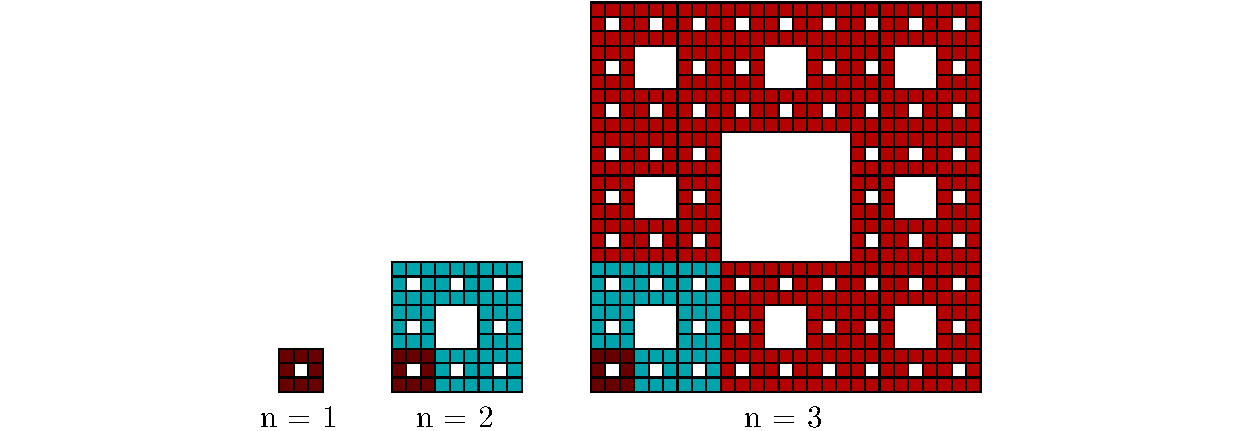
\includegraphics[width=0.9\columnwidth]{frac_iterative_SC.pdf} 
\caption[Iterative scheme for constructing Sierpiński carpet]{Iterative scheme for constructing Sierpiński carpet. Having a square lattice of the size $3^n \times 3^n$, we divide it in 9 smaller squares and remove the lattice sites within the central square. The process is then performed for remaining 8 squares and repeated as long as the smallest blocks are of a length $3$ with a one hole in the middle (are equivalent to the first-order generation of the carpet, $n = 1$).}
\label{fig:iterative-SC}
\end{figure}

Even though spectral properties of the SC and the SG were investigated before~\cite{GHEZ19871291,PhysRevB.29.5504, PhysRevLett.49.1194, PhysRevB.60.10054}, the topological aspects of the Hamiltonians defined on fractal lattices remain not fully explored. Only recently, results on BHZ model defined on fractal geometries were reported in Ref.~\cite{2018:BHZ} and the construction of spinless chiral $p-$ and $p +ip-$wave superconductors on the SC and the SG was discussed in Ref.~\cite{PaiFractal2019}. In particular, understanding the bulk-boundary correspondence in such systems is problematic as well as there is no sharp distinction between the bulk and the edge~\cite{EdgesFremling2020, KatnelsonFractal2020}. A final motivation to investigate Hamiltonians on fractals is related to the fractons. Fractonic topologically ordered models host fractionalized point-like excitations, fractons, which are immobile. In some of them (called type-II model), operators that create excitations have support on a fractal subset of the three-dimensional lattice. 

\begin{figure}[H]
\centering
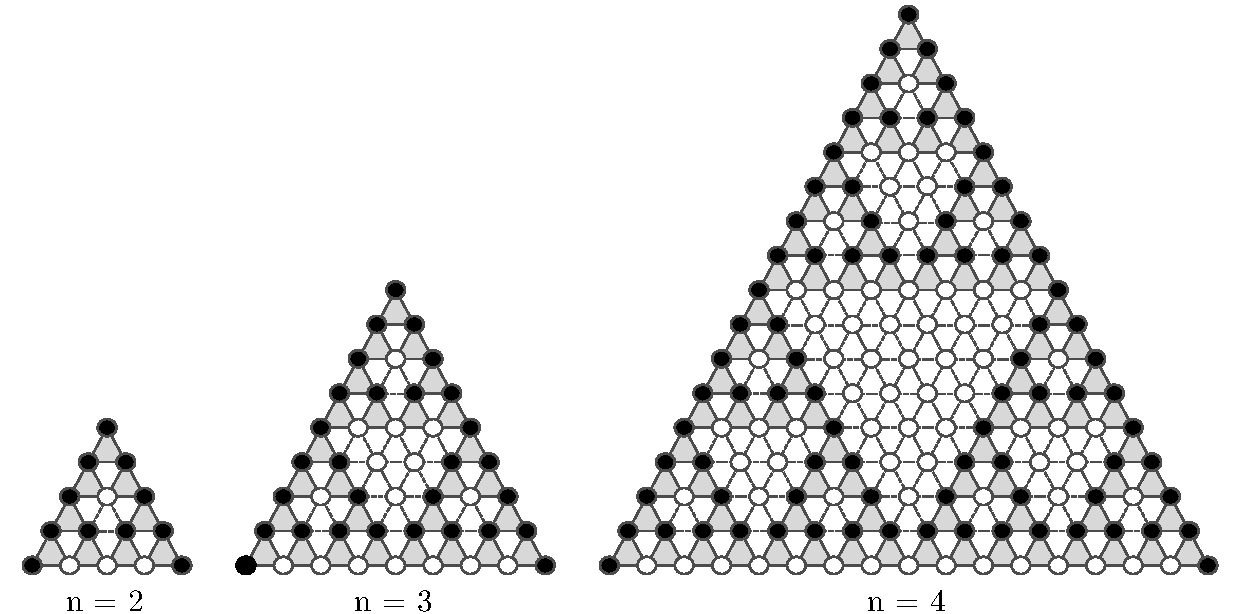
\includegraphics[width=0.9\columnwidth]{frac_iterative_SG.pdf} 
\caption[Iterative scheme for constructing Sierpiński gasket]{Iterative scheme for constructing Sierpiński gasket. To each site in a triangular lattice, we assign an integer and create a pattern which resembles the Pascal's triangle. If an associated value mod 2 is equal to one, then the site is filled with black color, otherwise is white; this procedure allows to determine which bonds have to be removed. For a white site located in $c$-th column and $r$-th row, three neighbouring hoppings are set to zero (denoted by a dashed black line): between white at $(c, r)$ and black ones at $(c-1, r + 1)$, $(c+1, r + 1)$, respectively, as well between black sites at $(c-1, r + 1)$ and $(c+1, r + 1)$. Matrix elements in the Hamiltonian corresponding to the completely disconnected lattice sites are then removed.}
\label{fig:iterative-SG}
\end{figure}

For instance, the integer quantum Hall effect can be seen as one of the most robust topological phases as it does not require any symmetries (some authors consider IQH states as invertible topologically ordered states with long-range entanglement~\cite{kong2014braided, freed2014shortrange}), but exists only in systems in even spatial dimensions\footnote{In odd dimensions, IQH states are equivalent to trivial band insulators.}. All band insulators without any symmetry constraints are topologically equivalent in 1D, thus a strong topological phase cannot exist, and the 3D version of IQHE can be only constructed as a weak phase whose properties are inherited from the two-dimensional realization~\cite{10foldRyu2010, PhysRevLett.93.206602}. Therefore, one may ask if quantum Hall states may be realized on almost two-dimensional lattices such as SC and SG. We firstly start with a short introduction to the lattice realization of the IQHE known as the Hofstadter model. After exemplifying the Hofstadter model on a square lattice, we then move to the investigations of this model on the lattice regularization of two aforementioned fractal geometries, \ie the Sierpiński-Hofstadter problem.

%%%%%%%%%%%%%%%%%%%%%%%%%%%%%%%%%%%%%%%%%%%%%%%%%%%%%%%%%%%%%%%%%%%%%%%%%%%%%%%%%%%%%%%%%%%%%%%%%%%%%%%%%%%%%%%%%%%%%%%%
\section{The Hofstadter model}
\label{sec:frac_model}
In the continuum limit, the quantum Hall effect is characterized by the macroscopically degenerated Landau levels and the quantized Hall conductivity which is directly linked to the number of occupied Landau levels. The essential properties of the IQHE can be captured by a simple tight-binding model of non-interacting electrons in a 2D periodic potential and in the presence of magnetic field. As one expects the electrons to be spin-polarized due to the magnetic field, we treat them effectively as spinless fermions. 

Let us first consider the model without an external field, which includes only nearest-neighbors terms
\begin{equation}
H =  - \sum_{\langle i, \, j \rangle} \left( t_x c^{\dagger}_{i+1, j } c_{i, j} + t_y c^{\dagger}_{i, j +1 } c_{i, j}  \right) + \mathrm{h.c.}
\label{tb:generic}
\end{equation} 
$c^{\dagger}_{i, j }$ and  $c_{i, j }$ are the electron creation and annihilation operators on the site labeled by $i$ and $j$, while $t_x$ and $t_y$ are the hopping terms between neighboring sites in the $x$ and $y$ directions, respectively. If a magnetic field $\mathbf{B}$ is applied perpendicularly to the lattice, $\mathbf{B} = B \hat{\mathbf{z}}$, all lattice plaquettes are penetrated by a magnetic flux $\Phi$. Using Stokes' theorem over a closed loop, we obtain a relation
\begin{equation}
\Phi = \int_{A} \mathbf{B} \cdot d \mathbf{S}  = \int_{A} ( \nabla \times \mathbf{A} ) \cdot d \mathbf{S}  = \int_{\partial A}  \mathbf{A} \cdot d \mathbf{l} 
\label{eq:stokes}
\end{equation}
with $\mathbf{A}$ being the electromagnetic vector potential around the loop enclosing the surface $A = a \times a$. Therefore, an electron travelling along a closed loop $\partial A$ acquires an Aharonov-Bohm phase factor of $\exp (2 \pi \mathrm{i} \Phi / \Phi_0)$, where $\Phi_0 = h / e$ is the magnetic flux quantum. Within the tight-binding approximation, the Aharonov-Bohm phase can be incorporated by employing the Peierls substitution~\cite{Peierls1933} in which all hopping terms $t_{ij}$ are multiplied by an appropriate phase factor
\begin{equation}
t_{ij} \rightarrow t_{ij} e^{2 \pi \mathrm{i} A_{ij} / \Phi_0}, \hspace*{1cm} A_{ij} = \int_i^j \mathbf{A} \cdot  d \mathbf{l}.
\label{eq:peierls}
\end{equation}
In the following, we choose the Landau gauge in which $\mathbf{A} = B x \hat{\mathbf{y}}$ and the Hamiltonian reads 
\begin{equation}
H = - \sum_{\langle i, \, j \rangle} \left( t_x c^{\dagger}_{i+1, j } c_{i, j} + t_y  e^{- 2 \pi \mathrm{i} \alpha \cdot i } c^{\dagger}_{i, j +1 } c_{i, j}  \right) + \mathrm{h.c.}
\label{eq:ham_landau_gauge}
\end{equation}

\begin{figure}
\centering
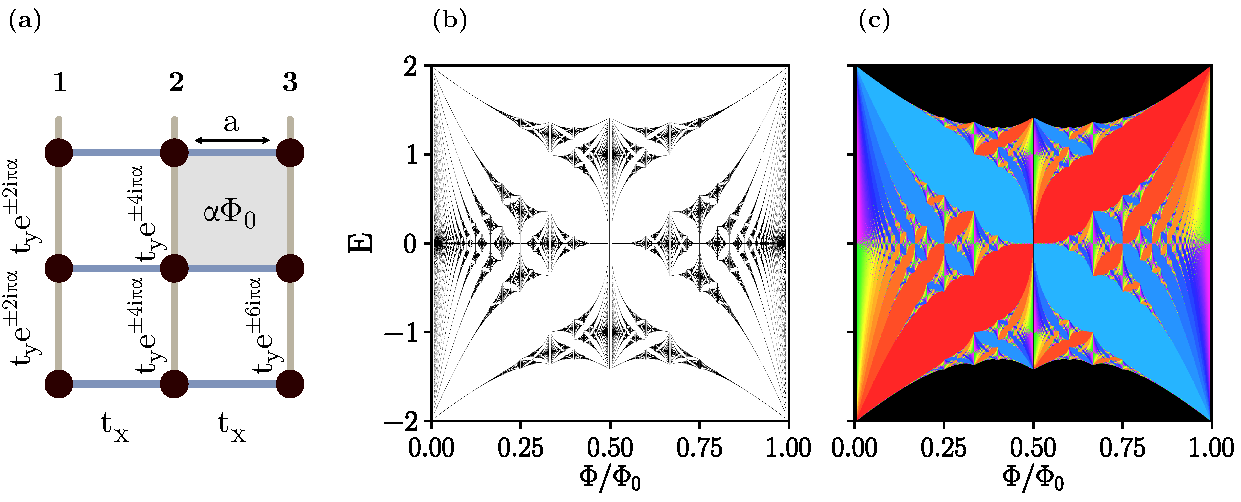
\includegraphics[width=0.95\columnwidth]{frac_hofstadter.pdf}
\caption[The Hofstadter model on a square lattice]{The Hofstadter model on a square lattice in the Landau gauge. \textbf{(a)} A schematic representation of hopping terms distribution on the lattice. Blue bonds correspond to the hoppings $t_x$ along $x$ direction and vertical grey bonds denote $t_y$ hoppings with a $x$-dependent phase factor $2 \pi \mathrm{i} \alpha \cdot x$. Each lattice plaquette (represented by a gray square of a size $a \times a$) is pierced by a magnetic flux $\Phi$ being a fraction $\alpha$ of the flux quantum $\Phi_0$. \textbf{(b)} Energy spectrum as a function of the magnetic flux $\alpha$ exhibits a self-similar pattern. The gapped regions can be colored by the corresponding Hall conductivity $\sigma_{xy}$ in units of $e^2 / h$ as pictured in \textbf{(c)}.}
\label{fig:square_hofstadter}
\end{figure}
 
This situation is depicted in Fig.~\ref{fig:square_hofstadter}~(a). If the values of the magnetic flux per plaquette $\alpha = \Phi / \Phi_0 = p / q$ are irrational, the energy spectrum consists of uncountably many points, which are all separated by finite gaps. The structure of the spectrum resembles the Cantor set\footnote{The Cantor set is an uncountable set of real numbers in the unit interval of measure zero and can be constructed recursively by dividing the unit interval into three equal intervals of length $1/3$ and then deleting the central one.}. For rational values of $\alpha$, where $p$ and $q$ are coprime integers, it is possible to define the magnetic unit cell being the smallest set of lattice plaquettes that encloses an integer number of flux quanta and transform the model into momentum space. The resulting Hamiltonian is not, however, translationally invariant with the translation operators of the underlying lattice. This is reflected by the fact that the Bloch Hamiltonian is not diagonal with respect to $k$ and there is a mixing between different $k$-sectors, $(k_x, k_y) \rightarrow (k_x \pm 2 \pi \Phi m, \, k_y)$ with $m$ being an integer running over $m = 0, \ldots, q-1$~\cite{bernevig2013topological}. It is possible, though, to define translations with a periodicity of one lattice site in the $y$ direction and $q$ lattice sites in the $x$ direction; as a consequence, the magnetic BZ is $q$ times smaller. Then, the Hamiltonian is 
\begin{equation}
H = \frac{a^2}{4 \pi^2} \int_{- \frac{\pi}{qa}}^{\frac{\pi}{qa}} \int_{- \frac{\pi}{a} }^{\frac{\pi}{a}} H(k_x, k_y) \, d k_x d k_y
\label{eq:hofstadter_bloch1}
\end{equation}
with
\begin{equation}
\begin{aligned}
H (k_x, k_y)  =  &-t_x  \left[ \sum_{m =0}^{q-1} e^{\mathrm{i} k_x a} a^{\dagger}_{k_x, \tilde{k_y} (m + 1)}   a_{k_x, \tilde{k_y} m} + e^{- \mathrm{i} k_x a}  a^{\dagger}_{k_x,\tilde{k_y} (m - 1)} a_{k_x, \tilde{k_y}  m} \right] \\
& -t_y \left[ \sum_{m =0}^{q-1} \cos(k_y a + 2 \pi \Phi m)  a^{\dagger}_{k_x,\tilde{k_y} m }   a_{k_x, \tilde{k_y}  m} \right] + \mathrm{h. c.} 
\end{aligned}
\label{eq:hofstadter_bloch2}
\end{equation} 
where $a^{(\dagger)}_{k_x, \tilde{k_y}}$ are new creation (annihilation) operators in reciprocal space with $\tilde{k_y} = k_y + 2 \pi \Phi$. For weak fields, the model reproduces Landau levels, but at larger values of $\Phi$ the energies proceed to broaden and the spectrum has a remarkable self-similar structure known as the Hofstadter's butterfly~\cite{1976:Hofstadter} (shown in Fig.~\ref{fig:square_hofstadter}~(b)). Such spectrum arises from the interplay between two competing length scales: one associated with the periodicity of a lattice potential (lattice constant $a$) and the magnetic length $l_B$ connected to the cyclotron radius of a uniform magnetic field. The key properties are:

\begin{enumerate}[label=\textbf{\arabic*.}]
\item The spectra for $\alpha$ and $\alpha + N$ (with $N \in \mathbb{Z}$) are identical; therefore, it is sufficient to study only the interval $\alpha  \in [0, 1]$.
\item The Bloch bands break up into $q$ distinct energy bands. If $q$ is odd, all the bands are separated by a gap, whereas for even $q$, all energy bands except the central two (which touch at $E = 0$) are separated by finite energy gaps.
\item Each Hofstadter band is topologically non-trivial and carries a non-zero Chern number.
\end{enumerate}

A relation between the fractal spectrum in the Hofstadter model and the Hall conductivity can be described by the Diophantine equation. Three positive integers $r$, $p$ and $q$ (where $p$ and $q$ are relatively prime) satisfy
\begin{equation}
p t_r + q s_r = r,
\label{eq:diophantine}
\end{equation}
where $t_r$ and $s_r$ depend on the value of $r$. The equation has a solution for $t_r, s_r \in \mathbb{Z}$ if and only if $r$ is a multiple of the greatest-common-divisor (GCD) of $p$ and $q$. Because $p$ and $q$ are coprime, GCD is then $1$ and Eq.~\eqref{eq:diophantine} has a unique solution if
\begin{equation}
0 \leq r \leq q, \hspace*{0.5cm} |t_r| \leq q / 2.
\end{equation}
For a fixed magnetic flux $p/q$, an argument due to \v{S}treda~\cite{Streda_1982} shows that such an equation must be satisfied by the Hofstadter model, with $r$ corresponding to the number of occupied bands (that is, the Fermi energy lies inside the $r$-th gap) and $t_r$ is the associated Hall conductivity in units of $e^2/h$
\begin{equation}
\sigma_{xy} = - \frac{e^2}{h} t_r.
\end{equation}
We illustrate the Hall conductivities associated with the energy gaps in Fig.~\ref{fig:square_hofstadter}~(c).

%%%%%%%%%%%%%%%%%%%%%%%%%%%%%%%%%%%%%%%%%%%%%%%%%%%%%%%%%%%%%%%%%%%%%%%%%%%%%%%%%%%%%%%%%%%%%%%%%%%%%%%%%%%%%%%%%%%%%%%%
\section{The Sierpiński-Hofstadter problem}
\label{sec:sierp-hof}
To define the topology of quantum states, only a notion of locality and the possibility to take a thermodynamic limit are required. Since it is possible to specify quantum states on general graphs, it is important to ask what type of properties a graph must have to host topological states. Here, we would like to address this question by examining Sierpiński carpet and gasket in a homogeneous magnetic field and ask whether the features similar to those in conventional quantum Hall systems are observed. 

Let us move to the Hofstadter model represented on the chosen fractal lattices with open boundary conditions (OBC). In general, it is possible to apply periodic boundary conditions (PBC) in both directions; for the carpet, the implementation is straightforward, but the gasket requires more attention\footnote{PBC can be realized, for instance, by representing the SG in a form of a rectangular triangle (which is topologically equivalent to the equilateral version), creating a mirror-symmetric copy with respect to its hypotenuse and treating two triangles together as a new, square-shaped system. The resulting structure has the same dimension $d_H$, but it may \emph{not} share other properties with the original gasket. An alternative construction was proposed in Ref.~\cite{PaiFractal2019}, where four gaskets are arranged on alternating faces of an octahedron, hence all lattice site have the same coordination number equal to four.}. Complex fractal pattern can be generated by an iterative procedure in which the system size increases with every step, but the distance between lattice sites remains the same. Such setting is most relevant to potential experiments on a nanoscopic scale as it introduces a natural cutoff. In order to construct the carpet, we start with a simple square lattice with $L (n) = 3^n$ sites along the outer edge, where $n$ is an iteration step. Then, in every step $n$, $ \left( 1 - ( 8 /9 )^n \right) \cdot 9^n$ lattice sites are removed (the procedure is illustrated in Fig.~\ref{fig:iterative-SC}). From the Pascal's triangle modulo $m$ (with $m$ being a prime number) embedded in a triangular lattice having $2^n + 1$ rows, it is possible to obtain a series of gasket-like lattices with $d_H = 1 + \log_m \left( \frac{m + 1}{2} \right)$ and the case of $m = 2$ corresponds to SG, which we demonstrate in Fig.~\ref{fig:iterative-SG}.

Through the work, we consider the tight-binding Hamiltonian
\begin{equation}
H = -t  \sum_{\langle i, j \rangle} e^{\mathrm{i} A_{ij}} c^{\dagger}_i c_j + \mathrm{h.c.},
\label{eq:frac_ham}
\end{equation}
with the vector potential satisfying relation $\mathbf{B} =  \nabla \times \mathbf{A}$ and the phase factors distribution presented in Fig.~\ref{fig:flux_distr}. The hopping integral $t$ between nearest-neighbors is the only energy scale in the model and it is set to $t = 1$.  We assume that the magnetic field is homogeneous in the two-dimensional space in which the fractal lattice is embedded. The magnetic flux per smallest element of lattice-regulated versions of carpet and gasket (that is, the smallest square in the SC and the smallest triangle for the SG) is chosen to be $\Phi$.

\begin{figure}[H]
\centering
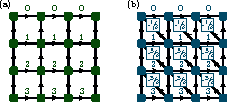
\includegraphics[width=0.9\columnwidth]{frac_flux.pdf} 
\caption[Vector potential gauge choice for fractal lattices]{Phase distribution on $4 \times 4$ \textbf{(a)} square and \textbf{(b)} triangular lattices with open boundary conditions. $A_{ij}$ phase between sites $i$ and $j$ is equal to the number shown above the bond in $2 \pi$ units. A phase acquired with the respect to the direction pointed by arrows has a positive sign.}
\label{fig:flux_distr}
\end{figure}

%%%%%%%%%%%%%%%%%%%%%%%%%%%%%%%%%%%%%%%%%%%%%%%%%%%%%%%%%%%%%%%%%%%%%%%%%%%%%%%%%%%%%%%%%%%%%%%%%%%%%%%%%%%%%%%%%%%%%%%%
\subsection{Spectral properties}
\label{sec:frac_spectral}
Firstly, let us focus on the energy spectra obtained by diagonalizing the Hamiltonian given in Eq.~\eqref{eq:frac_ham} for different values of the magnetic flux. To describe the number of single-particle states within a given energy window $[ \epsilon, \epsilon + \delta]$ that electrons are allowed to occupy, we compute the density of states (DOS) 
\begin{equation}
D(\epsilon) = \sum_{\lambda = 1}^N \delta \left (\epsilon - E_{\lambda} \right)
\label{eq:dos}
\end{equation}
for sets of energy levels $E_\lambda$. Discrete DOS spectra can be smoothed using a Gaussian function, hence Eq.~\eqref{eq:dos} can be rewritten as
\begin{equation}
D(\epsilon, \alpha) = \sum_{\lambda} \exp  \left\{ - \left[ \epsilon - E_{\lambda} (\alpha) \right]^2 / \eta \right\}
\label{eq:dos_gauss}
\end{equation}
with a broadening parameter $\eta$ and $\alpha = p /q$. In Fig.~\ref{fig:frac_spect}~(a, d), we show DOS (with $\eta = 0.001$) for the SC at iteration $n = 4$ and the SG at iteration $n = 6$ with open boundary conditions. As in case of regular lattices, a presence of magnetic field gives rise to the Hofstadter's butterfly~\cite{1976:Hofstadter}. 

The spectrum of the SC (see Fig.~\ref{fig:frac_spect}~(a)) is reflection-symmetric with respect to the $E = 0$ and the $\alpha = 1/2$ lines due to a chiral symmetry of the Hamiltonian on this bipartite lattice. The spectrum is mostly gapless, but two finite gaps of maximal extend in energy $\sim 0.1$ are observed for small range of the flux around $\alpha = 1/4, \, 3/4$ and $E = 0$. Regions of low DOS host states with distinct localization properties, which are discussed in more details in Section~\ref{sec:frac_edgemodes}. If PBC are assumed, these regions are gapped with a few states in the middle of gaps (appearing as thin yellow branches in dark blue areas in Fig.~\ref{fig:frac_spect}~(a)).

Fig.~\ref{fig:frac_spect}~(d) shows the spectrum of the SG, which has only a point-inversion symmetry about $\alpha=1/2$ and $E=0$, while reflection symmetries are lost for this non-bipartite lattice. Various fully gapped regions are observed and large DOS appears around two points: $\alpha = 1/4$, $E \approx 1.4$, together with a symmetry-related point $\alpha = 3/4$, $E \approx -1.4$. It is known that at zero flux the spectrum is fractal and the energy levels are macroscopically degenerated~\cite{PhysRevB.28.3110}; introducing a finite field leads to lifting this degeneracy. This degeneracy is mostly visible around $E = 2$ and $E = \pm 1$.

\begin{figure}[H]
\centering
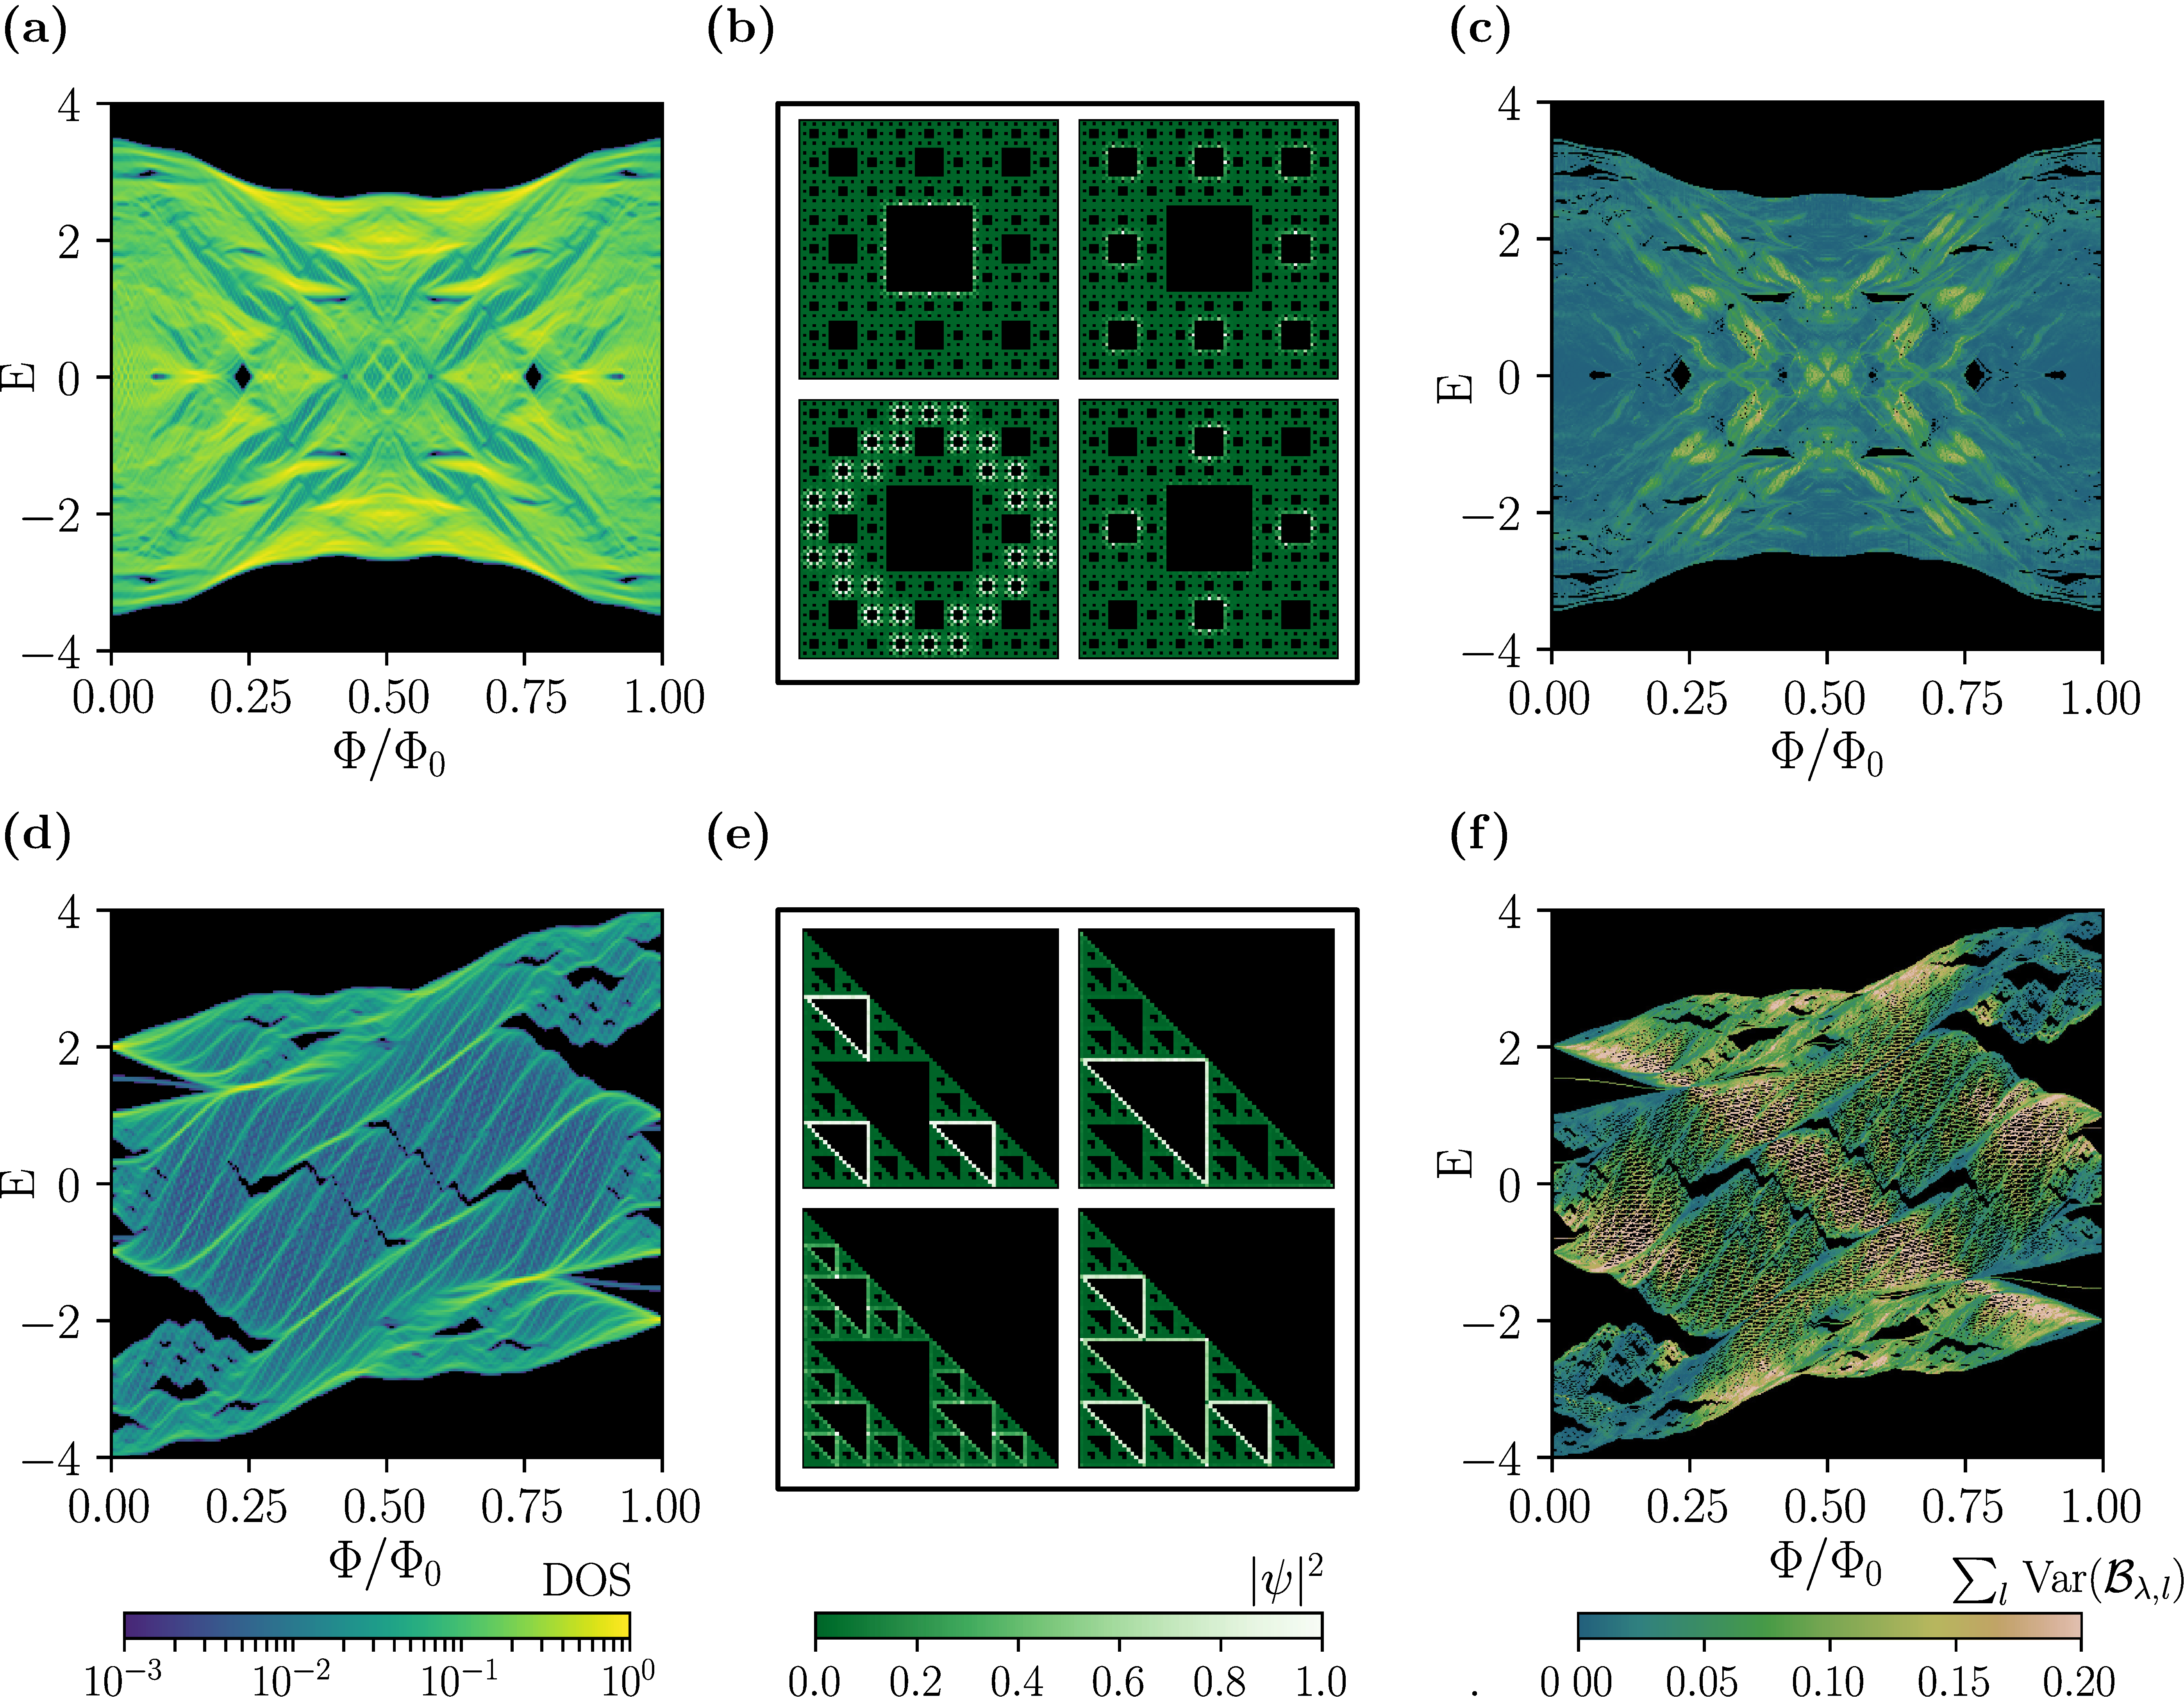
\includegraphics[width=\textwidth]{frac_spectra.pdf} 
\caption[Spectral and eigenstate localization properties of Sierpiński carpet and gasket]{\textbf{(a, d)} Density of states in the energy-flux plane, \textbf{(b, e)} localization of the eigenstates, and \textbf{(c, f)} edge-locality marker. Low DOS regions are represented by dark blue color. Two energy gaps at $E = 0$ are seen for SC, while the energy spectrum of SG exhibits numerous gaps. Representative electronic densities at time-reversal symmetric point ($\alpha = 1/2$) around $E = 0$ are presented in \textbf{(b, e)} and the color scale corresponds to the square modulus $| \psi_i|^2$ of the wave function normalized by its maximum value. $\mathcal{B}_{\lambda, l}$ marker shown in \textbf{(c, f)} quantifies the changes in localization properties between consecutive eigenstates at fixed flux. Parts of the spectra with smaller density are associated with largely varying values of edge-locality marker.}
\label{fig:frac_spect}
\end{figure}

%%%%%%%%%%%%%%%%%%%%%%%%%%%%%%%%%%%%%%%%%%%%%%%%%%%%%%%%%%%%%%%%%%%%%%%%%%%%%%%%%%%%%%%%%%%%%%%%%%%%%%%%%%%%%%%%%%%%%%%%
\subsection{Edge modes}
\label{sec:frac_edgemodes}
A striking feature of a standard integer quantum Hall setup is the existence of protected edge modes. As the distinction between bulk and boundaries in fractal lattices is not sharp, it is not enough to simply point out that the edge modes are present. Hence, we would like to investigate the localization properties of the eigenstates in more details. Previous studies of fractal lattices suggested~\cite{supp1, supp2} that introducing a magnetic field leads (on average) to the delocalization of eigenstates. This observation can be confirmed by computing inverse participation ratio (IPR)
\begin{equation}
I_{\psi} = \frac{\sum_i | \psi_i |^4}{\left(\sum_i  |\psi_i |^2 \right)^2}, 
\label{eq:ipr}
\end{equation}
for any wavefunction expandable in the real space basis $\ket{\psi} = \sum_i \psi_i \ket{i}$. The IPR takes values between 1 and the inverse of the number of sites $N$, where 1 corresponds to a perfect localization at one site and $1/N$ to evenly distributed weights over all lattice sites. At zero flux $\alpha = 0$ (Figs.~\ref{fig:IPR_SC}~(a) and~\ref{fig:IPR_SG}~(a)), the distribution of IPRs is peaked close to the inverse of the number of sites belonging to the edges of the second-smallest squares or triangles. For a finite field, the distribution of IPRs shifts to smaller, \ie, more delocalized values. This effect is more apparent for the SC compared to the SG.

\begin{figure}[H]
\centering
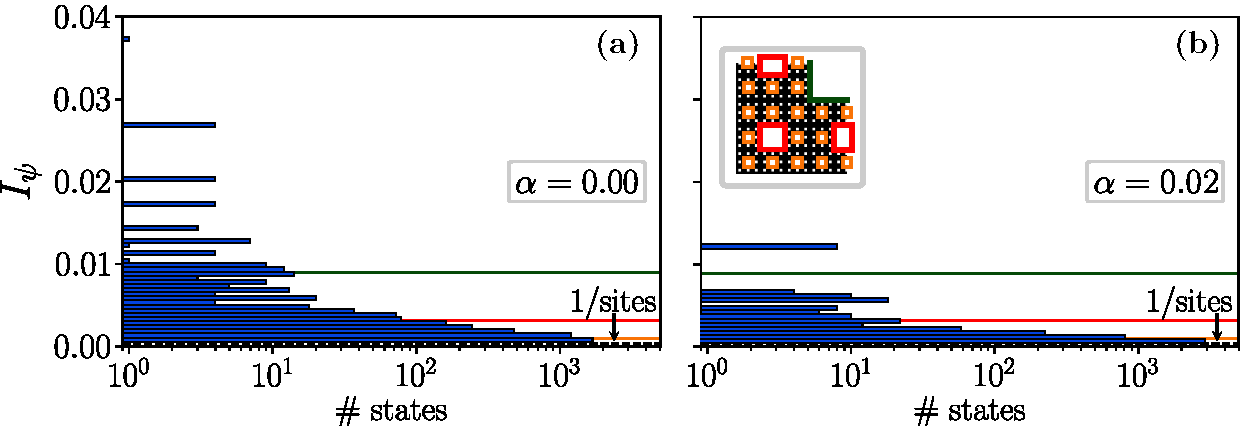
\includegraphics[width = 0.95\columnwidth]{frac_iprSC.pdf}
\caption[Distribution of IPR for the Sierpiński carpet]{Distribution of IPR for the Sierpiński carpet: at \textbf{(a)} $\alpha = 0$ and \textbf{(b)} $\alpha = 0.02$. Inset presents a close-up of the carpet with the internal edges of different hierarchies marked with different colors. A finite magnetic field leads to the delocalization of the eigenstates.}
\label{fig:IPR_SC}
\end{figure}

\begin{figure}[H]
\centering
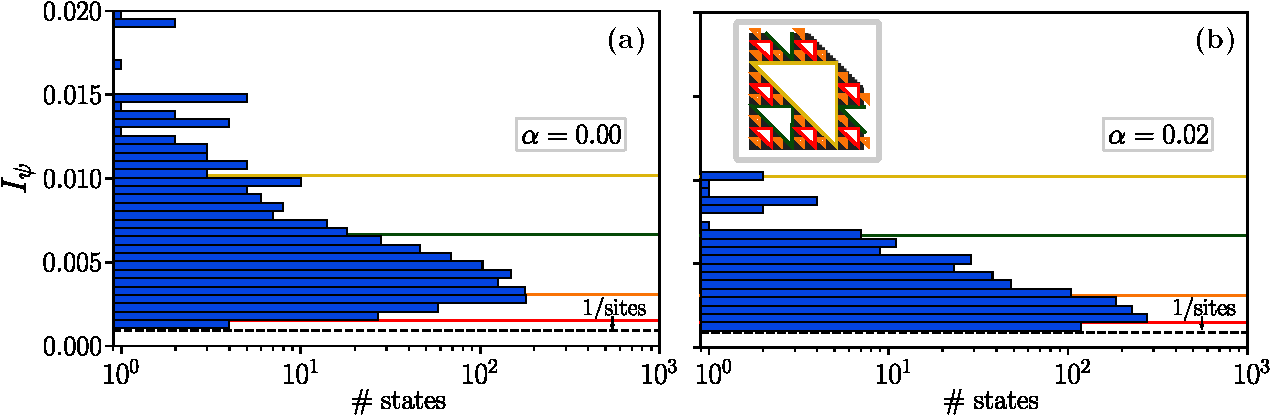
\includegraphics[width = 0.97\columnwidth]{frac_iprSG.pdf}
\caption[Distribution of IPR for the Sierpiński gasket]{Distribution of IPR for the Sierpiński gasket at \textbf{(a)} $\alpha = 0$ and \textbf{(b)} $\alpha = 0.02$. Inset displays a close-up of the gasket with the highlighted edges of different hierarchies. Similar to the carpet, the distribution of IPRs is shifted towards more delocalized values for the non-zero magnetic field.}
\label{fig:IPR_SG}
\end{figure}

Remarkably, by contrasting the case of zero and non-zero magnetic field, we observe an intriguing change in the character of the most localized states. Fig.~\ref{fig:frac_spect}~(b, e) shows the electronic densities for the eigenstates at the time-reversal symmetric point ($\alpha = 1/2$) around zero energy. States are sharply localized at the internal edges of the fractal at different levels of the hierarchy and they can be found in very close spectral proximity to one another in various places of the phase diagram at finite magnetic field. Conversely, at zero magnetic field, the most localized states exhibit complex interference pattern, but are usually not supported on internal edges. To quantify the degree of localization, we compute edge-locality marker defined as
\begin{equation}
\mathcal{B}_{\lambda, l} = \sum_{i \in \mathcal{E}_l} | \psi_{\lambda,i} |^2, 
\label{eq:edgemarker}
\end{equation}
where $\braket{i | \psi_{\lambda}} = \psi_{\lambda,i} $ and the summation is taken over the edges $\mathcal{E}_l$ of all internal squares or triangle at level $l$ of the hierarchy such that $l = 0$ corresponds to the lattice sites along all smallest squares/triangles and $l = n$  - to the outermost edge. Hence, $\mathcal{B}_{\lambda, l}$ measures how much an eigenstate $\ket{\psi_{\lambda}}$ with an energy $E_{\lambda}$ has a support on the different edges of level $l$. With every state $\ket{\psi_{\lambda}}$, we associate a set of $\mathcal{B}_{\lambda, l}$ for $l = 0, \ldots, n$. In order to detect where in the phase diagram the localization properties are varying the most, we compute the variance for each entry of the set $\mathcal{B}_{\lambda, l}$ across three states with energies $E_{\lambda - 1}$, $E_{\lambda}$ and $E_{\lambda+1}$, and sum these variances over $l$: $\sum_l \mathrm{Var} \left( \lbrace \mathcal{B}_{\lambda - 1, l}, \mathcal{B}_{\lambda, l}, \mathcal{B}_{\lambda + 1, l} \rbrace \right)$. In regular lattices, peaks of the variance separate bulk states from edge states. Results shown in Fig.~\ref{fig:frac_spect}~(c, f) indicate that sharp changes in eigenstate localization appear mostly in the low DOS regions, thus we can interpret these regions as made of edge-like states at various levels of the fractal hierarchy.   

\subsection{Real-space formulation of topological invariants}
Due to the lack of translational invariance, it is not possible to compute topological indices based on a bundle of occupied Bloch states. However, we may employ a real-space perspective on obstructions of filled states in a topological system. Non-zero topological index implies the existence of extended edge modes, therefore it is not possible to perturb the Hamiltonian such that it would lead to the exact localization of all the occupied states without breaking the symmetries or closing the gap (otherwise it would mean that the system is topologically trivial). This can be captured by using non-commutative geometry, which allows to define appropriate indices for each symmetry classes~\cite{2011:Prodan}. 

\subsubsection{Bott index}
The Bott index, introduced in the context of condensed matter physics by Loring and Hastings~\cite{BottIdx}, tells whether a pair of unitary matrices can or cannot be approximated by a pair of commuting unitary matrices. In our case, we measure the commutativity of the projected position operators~\cite{LORING2015383}. A degree of commutativity of these operators is directly related to the localization properties of the Wannier functions: a vanishing Bott index implies the existence of exponentially localized Wannier functions with a spread being small compared to the linear size of the system~\cite{HASTINGS20111699, monaco2016localization}. A system that admits a representation in terms of exponentially localized Wannier functions has no strong topology, hence non-zero Bott index marks a non-trivial bulk topology.

Let us now define the Bott index and discuss its properties. Consider a representation of the position operators $X$ and $Y$, defined as
\begin{equation}
X_{ij} = x_i \delta_{ij} \hspace*{0.5cm} \mathrm{and} \hspace*{0.5cm} Y_{ij} = y_i \delta_{ij}.
\end{equation}
Given the linear size of the system $L$ and the coordinates rescaled to fit the interval $[0, 1)$, $X \rightarrow X / L$ and $Y \rightarrow Y/ L$, one constructs the matrices $U$ and $V$
\begin{equation}
\begin{aligned}
U &= P e^{i 2 \pi X} P  - (1 - P), \\ 
V &= P e^{i 2 \pi Y} P - (1 - P)
\end{aligned}
\end{equation}
and computes their product using the formula
\begin{equation}
B = \frac{1}{2 \pi} \mathrm{Im} \left( \mathrm{Tr} \, [ \log (V U V^{\dagger} U^{\dagger} ) ] \right), 
\label{eq:bott}
\end{equation}
where $P = \sum_{E < E_F} \ket{\psi} \bra{\psi} $ is the orthogonal projector on the occupied bands below the Fermi energy $E_F$. If the Hamiltonian is short-ranged and $E_F$ lies in a (mobility) gap, then the corresponding $P$ operator is also local. Note that $(1-P)$ term appears if the system has boundaries or when the projector $P$ onto the occupied subspace does not create an orthonormal basis~\cite{loring2019guide}. $U$ and $V$ matrices are approximately unitary, $U U^{\dagger} \approx \mathbb{1}$ and $V V^{\dagger} \approx \mathbb{1}$, and almost commute, $[U, V] \approx 0$, if $E_F$ is in a mobility gap; this indicates that $V U V^{\dagger} U^{\dagger}$ is then close to the identity.

We see that from the property $\det (V U V^{\dagger} U^{\dagger}) = \exp  \left( \mathrm{Tr} \left[ \log (V U V^{\dagger} U^{\dagger}) \right] \right)$ and $2 \pi \mathrm{i}$ periodicity of the complex exponential, we can write
\begin{equation}
\mathrm{Tr} \left[ \log (V U V^{\dagger} U^{\dagger} }) \right] = \log \left[ \det \left( V U V^{\dagger} U^{\dagger}  \right) \right] + 2 \pi \mathrm{i} m,  \hspace*{0.5cm}  m \in \mathbb{Z}.
\label{eq:bott_quant}
\end{equation}
For unitary matrices, $|det(V U V^{\dagger} U^{\dagger})| = 1$, hence $ \log \left[ \det \left( V U V^{\dagger} U^{\dagger}  \right) \right]$ vanishes and therefore the Bott index defined in Eq.~\eqref{eq:bott_quant} must be an integer. The Bott index is equal to zero if and only if $U$ and $V$ are (close to) a pair of commuting unitaries. If an eigenvalue of $ V U V^{\dagger} U^{\dagger}$ is far from the branch cut of the logarithm (chosen to be the negative real axis), the value of $B$ is not affected. However, if one of the eigenvalues crosses the branch cut, its phase changes by $2 \pi$ and therefore the Bott index changes. It has been proven that for gapped, short-ranged Hamiltonians, the Bott index is equivalent to the Chern number in the thermodynamic limit~\cite{toniolo2017equivalence, PhysRevA.96.023610}. Also, its applicability has been extended to the spinful systems, where the spin Bott index is defined analogously to the spin Chern number computed for two spin sectors separately~\cite{PhysRevLett.121.126401}. Therefore, we expect non-zero values of $B$ in the parts of spectrum hosting topologically non-trivial states.

Stability of the computation of the Bott index can be ensured by performing a singular value decomposition (SVD) of the $U$ and $V$ matrices, $U = Z_U \Sigma_U W_U^{\dagger}$ and $V = Z_V \Sigma_V W_V^{\dagger}$~\cite{PhysRevB.98.235425, PhysRevB.98.125130}
\begin{equation}
\begin{aligned}
U & \rightarrow \tilde{U} = Z_U W_U^{\dagger}, \\
V & \rightarrow \tilde{V} = Z_V W_V^{\dagger}.
\end{aligned}
\end{equation}

$\tilde{U}$ and $\tilde{V}$ matrices are unitary, because $Z$ and $W$ are unitary by definition, and the commutativity of the operators is preserved. 

Motivated by the application of the Bott index to fractal lattices~\cite{2018:BHZ}, we compute $B$ as a function of magnetic flux at different Fermi levels. The resulting phase diagrams are presented in Fig.~\ref{fig:bott_idx}, where numerous regions of non-zero $B$ are observed. We focus on the third generation of the carpet and $n =5$ iteration for the gasket as numerical efficiency of the Bott index is rather restricted to small system sizes. Nevertheless, in case of SC low DOS regions are in agreement with $B \pm 1$. Larger values of $B$ can be seen for fluxes around $ \alpha = 0.4 $ and $\alpha = 0.6$ at $E = 0$. For SG, a region with consistently non-zero Bott index corresponds to the part of the spectrum with sharp changes in eigenstate localization properties. This is in agreement with the picture of the low DOS regions being the equivalent of bulk-gapped energy regions hosting edge states in conventional topological systems.

\begin{figure}[H]
\centering
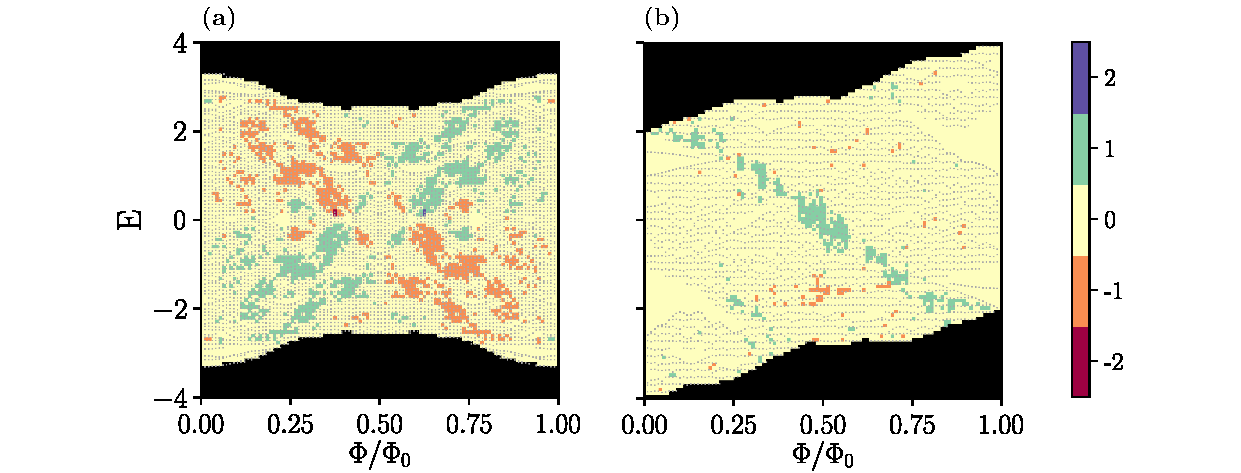
\includegraphics[width=\textwidth]{frac_bott.pdf}
\caption[Bott index at different Fermi levels as a function of magnetic flux]{Bott index at different Fermi levels as a function of magnetic flux for \textbf{(a)} carpet with $n = 3$ and \textbf{(b)} gasket with $n = 5$. Overlaying small grey dots denote the energy spectrum. In case of the carpet, low DOS regions overlap with non-zero Bott index in the phase diagram; additionally, small regions with $B = \pm 2$ are observed around $E = 0$ and fluxes $\alpha \sim 0.4, \, 0.6$. For the gasket, an extended region with $B = 1$ coincide with a set of states having largely varying localization properties.}
\label{fig:bott_idx}
\end{figure}

\subsubsection{Chern number}
A more efficient approach to compute real-space topological invariants is rather based on \emph{local} markers, which allows to investigate larger systems. Instead of performing the calculations for a full lattice, it is enough to consider the local index computed over the finite patch. If this patch is chosen to be far from the edges, then the result is insensitive to boundary conditions. We hence employ the real-space formula for the Chern number based on an antisymmetric product of projection operators $P$~\cite{KITAEV20062}, defined in the previous section
\begin{equation}
\mathcal{C} = 12 \pi \mathrm{i} \sum_{j \in A} \sum_{k \in B} \sum_{l \in C} \left( P_{jk} P_{kl} P_{lj} - P_{jl} P_{lk} P_{kj} \right),
\label{eq:chern_real}
\end{equation}
where $j, \, k, \, l$ label the lattice sites in three distinct neighboring sectors $A$, $B$ and $C$ arranged in a counterclockwise manner (consult Fig.~\ref{fig:lattice}). As a remark, for a translational invariant case, Eq.~\eqref{eq:chern_real} reduces to
\begin{equation}
\mathcal{C} = 2 \pi \mathrm{i} \mathrm{Tr} \left( P \left[ [X, P], [Y, P] \right] \right)
\label{eq:chern_real_translational}
\end{equation}
with $X$ and $Y$ being the operators of $x$ and $y$ coordinates, respectively, and the trace is taken over the unit cell. The sum in Eq.~\eqref{eq:chern_real} should converge to an integer, when the summation region is large enough. If $\mathcal{C}$ is indeed quantized, it becomes then independent of the detailed choice of $A$, $B$, $C$ in the limit where the number of sites in each part goes to infinity.

\begin{figure}[H]
\centering
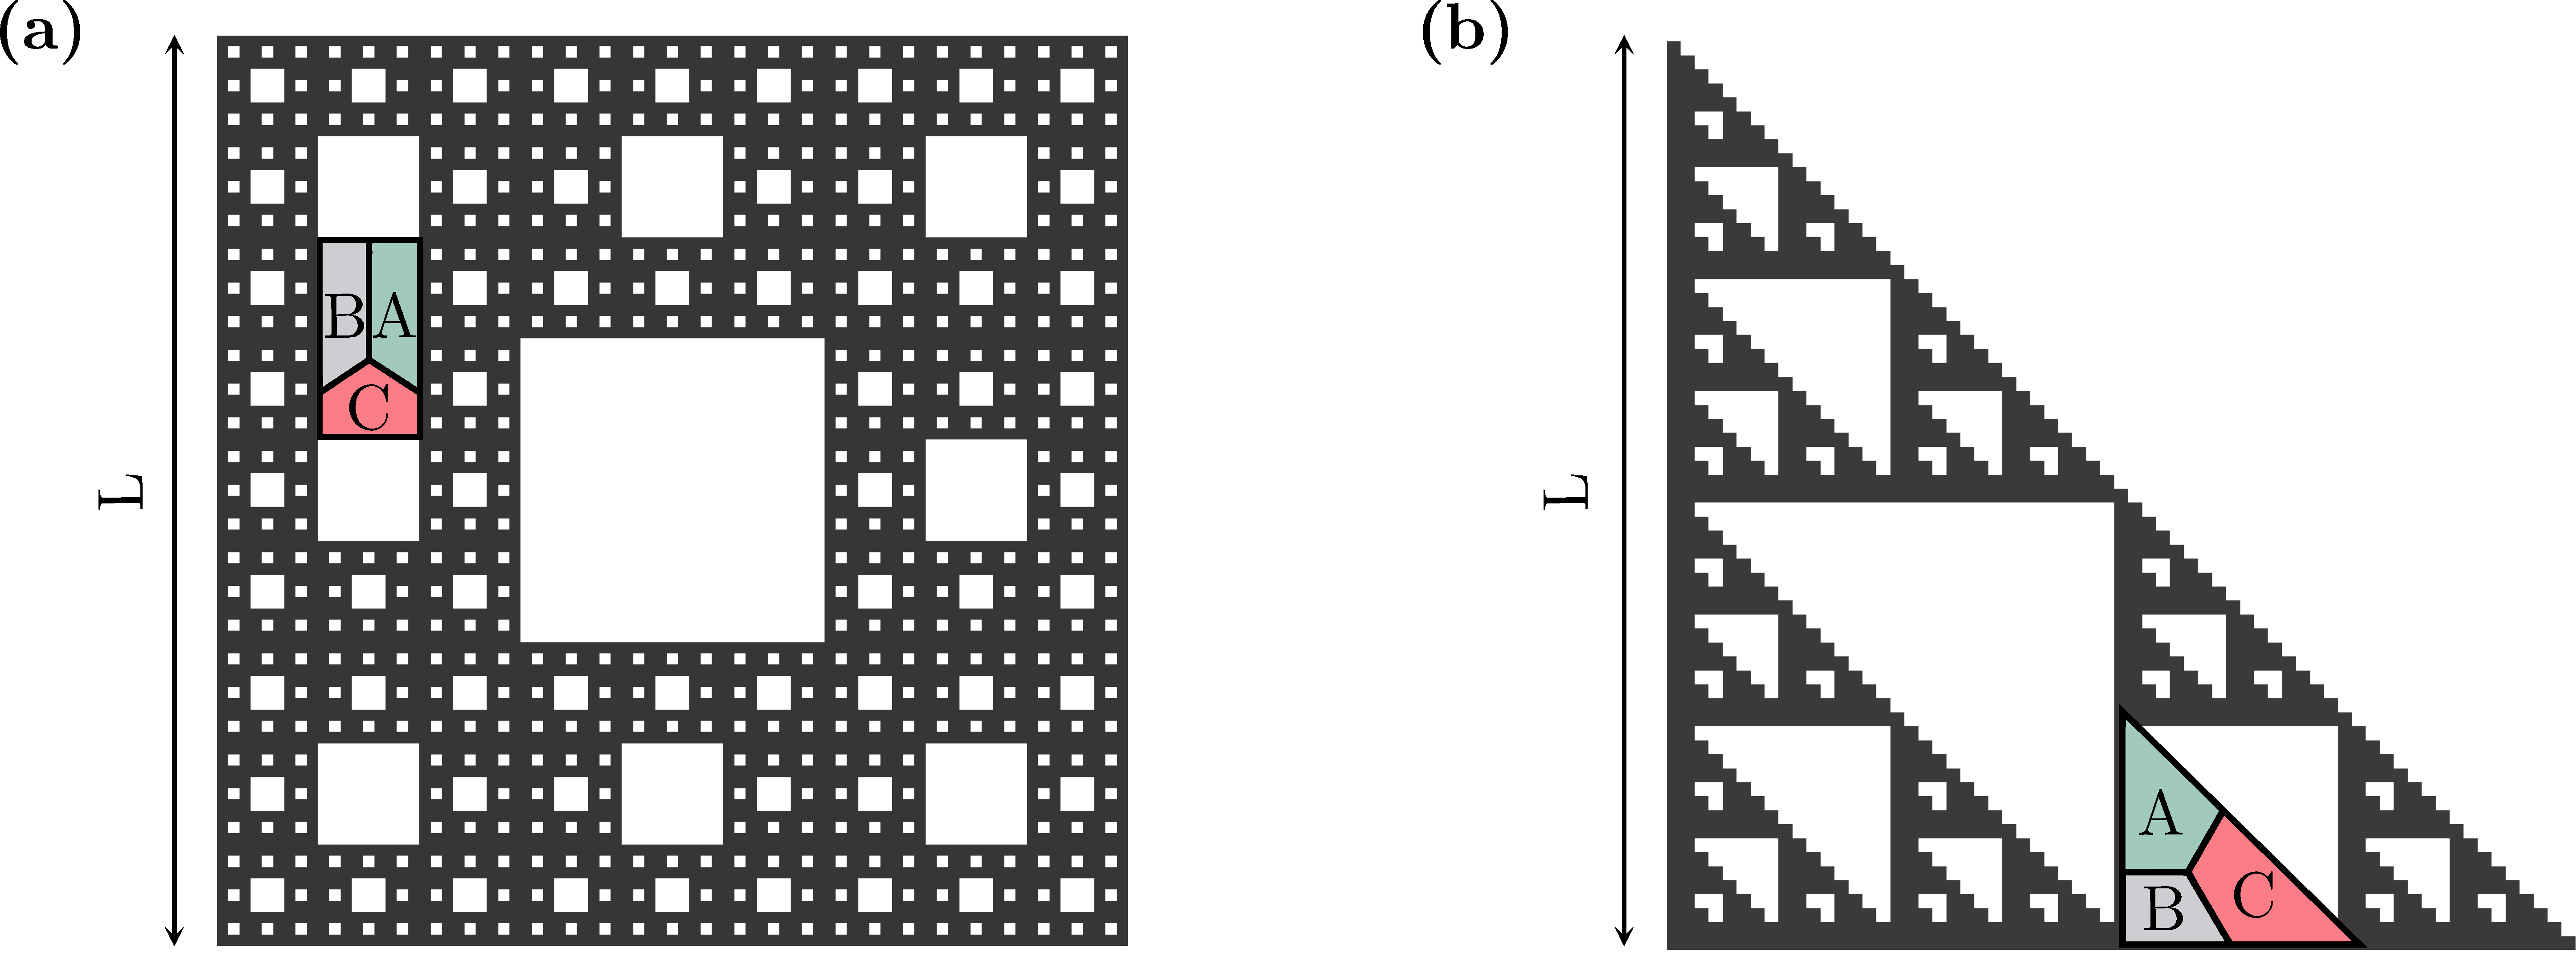
\includegraphics[width=0.95\columnwidth]{frac_lattice.pdf}
\caption[Lattice regularization of Sierpiński carpet and gasket]{\textbf{(a)} The fourth iteration of the Sierpiński carpet with $L = 81$ and \textbf{(b)} the sixth iteration of the Sierpiński gasket with $L = 65$. Black squares depict the lattice sites which are kept from the underlying regular square (in case of the carpet) and triangular (gasket) lattices. Summation regions used in real-space Chern number calculations are labeled with A, B, C.}
\label{fig:lattice}
\end{figure}

Using the SC as an example, in Fig.~\ref{fig:ChernScaling} we show how a real-space patch choice affects the quantization of $\mathcal{C}$. We compute $\mathcal{C}$ while varying the distance $R$ between the center and the corners of the patch that makes up $A$, $B$, $C$ sectors and keeping the aspect ratio of rectangle constant. When the summation region is too small or too large (close to the size of the entire system), $\mathcal{C}$ is far from a non-zero quantized value as expected. We focus on two Fermi levels, $E_F = -1.2$ and $E_F = -1.0$, which correspond to spectral regions with less and more quantized $\mathcal{C}$, respectively. For $E_F = -1.0$ which lies in low DOS region, $\mathcal{C}$ is very close to 1 over a large range of $R$. Conversely, for $E_F = -1.2$ (at large DOS), where $\mathcal{C}$ is not quantized, a strong $R$-dependence is found.

\begin{figure}[H]
\centering
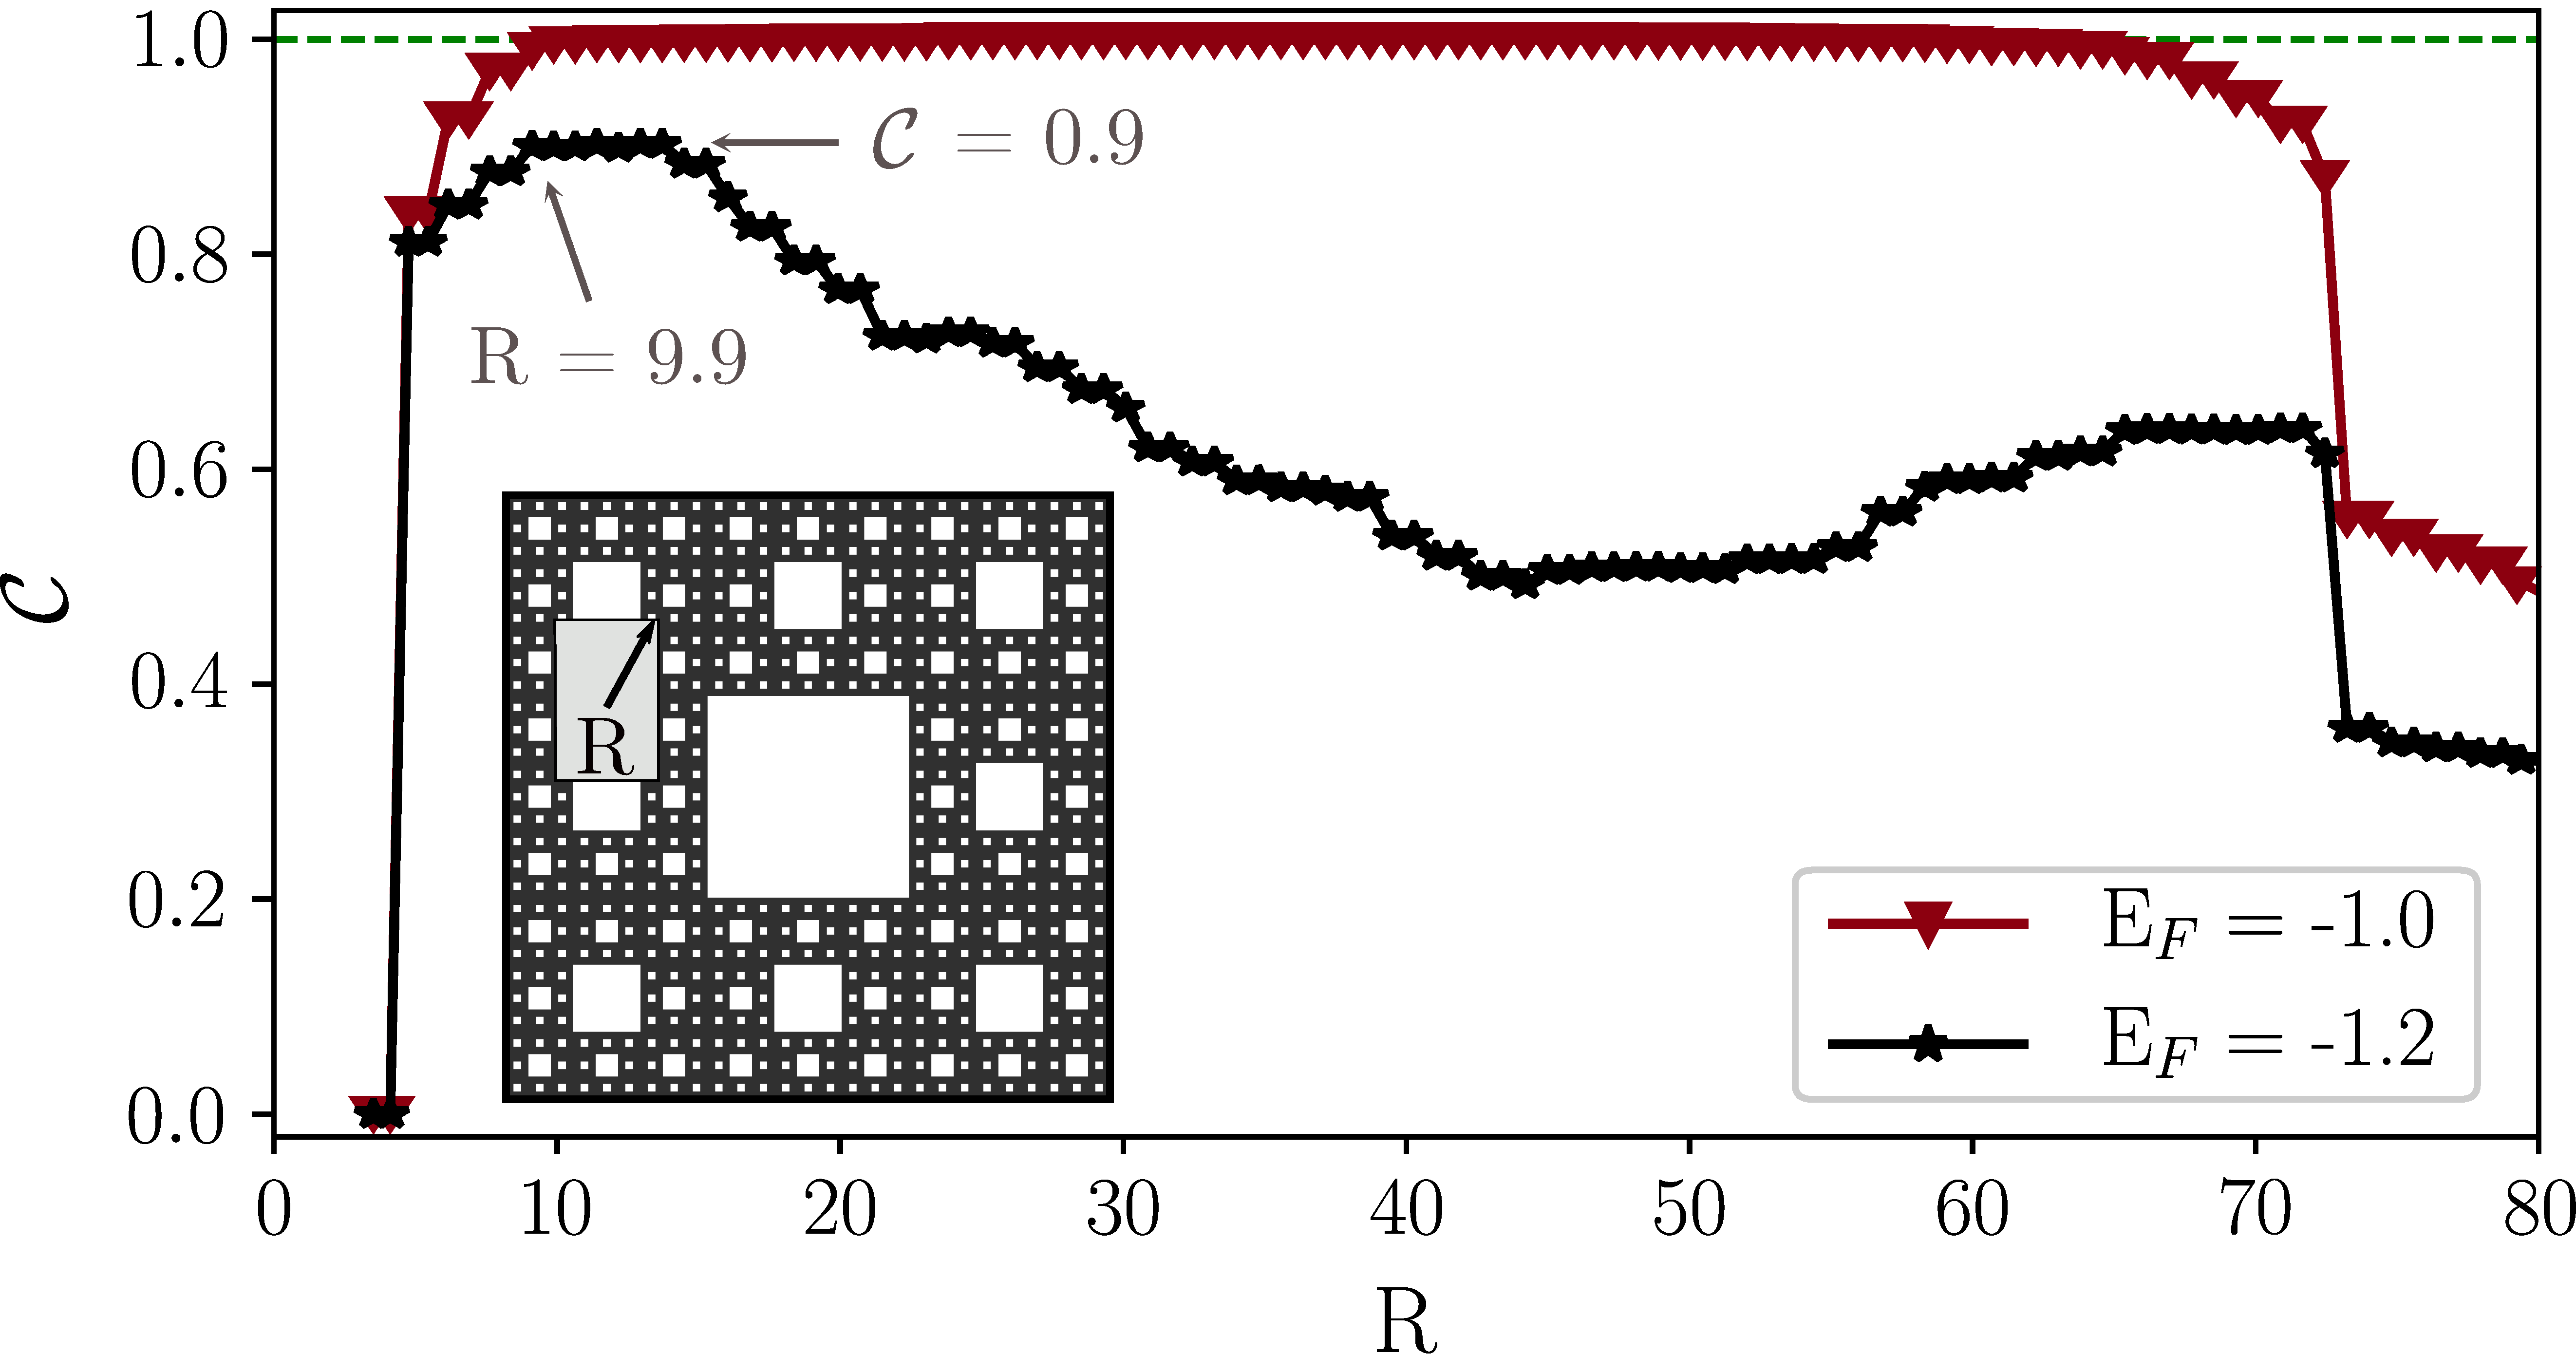
\includegraphics[width =0.8\columnwidth]{frac_chern_scaling.pdf}
\caption[Scaling of the Chern number with respect to a real-space patch size]{Real-space Chern number calculations for Sierpiński carpet as a function of the half of the diagonal of a rectangular patch $R$ for two Fermi levels $E_F = -1.2$ and $E_F = -1.0$ at fixed flux $\alpha = 1/4$. For spectral regions exhibiting stable plateaus with quantized $\mathcal{C}$, this quantization is observed for a large range of patch sizes. In case of large DOS regions, in which we dominantly observe deviation from a quantized value of $\mathcal{C}$, the value of $\mathcal{C}$ is sensitive to the size and shape of the summation region. $R = 9.9$ corresponds to the size of the patch shown in Fig.~\ref{fig:lattice}~(a).}
\label{fig:ChernScaling}
\end{figure}

Figs.~\ref{fig:frac_SC}~(d) and \ref{fig:frac_SG}~(d) present $\mathcal{C}$ as a function of the Fermi energy $E$ at fixed value of flux $ \alpha =1/4$ for the $n=4$ iteration of SC and the $n=6$ iteration of the SG with a patch size corresponding to the most robust results. We arrive at following conclusions:
\begin{enumerate}[label=\textbf{\arabic*.}]
\item All fully gapped regions of the spectrum, for both lattices, carry $\mathcal{C}=0$. Similar to the systems defined on regular lattices, an absence of in-gap states indicates that there are no topological edge modes\footnote{Not all edge states appearing in the bulk band gap are topological; protected edge states arising from a non-trivial bulk topology exhibit \emph{spectral flow} -- they interpolate across the energy gap and spectrally connect the conduction band with the valence band.}.

\item Low DOS regions for the SC in Fig.~\ref{fig:frac_spect}~(a) are associated with stable plateaus $\mathcal{C} \sim \pm 1.0$ (for a wide range of energies $E = -1.5 \ldots - 0.9$ and $E = 0.9 \ldots 1.5$), as well less quantized regions with $\mathcal{C} \sim \pm 0.96$ ($E = -2.6\ldots -2.5$ and $E = 2.5\ldots 2.6$). Deviations from quantized Chern numbers are observed when the DOS is enhanced, for example around $E = -1.2$ and $E = 1.2$. This suggests that edge modes are indeed chiral and contribute to the Chern number. In Refs.~\cite{2018:BHZ, PaiFractal2019}, the authors studied a wave packet evolution in different models on the SG and found that the chirality of wave packets initialized on any of the inner edges is opposite to the case when the wave packet propagates along the outermost edge. Such situation is also expected in our case.

\item Identification of non-trivial regions for the SG is less clear, yet a plateau from $E = 1\ldots 1.6$ converges to $\mathcal{C} \sim 1.0$. 
\end{enumerate}

\begin{figure}[H]
\centering
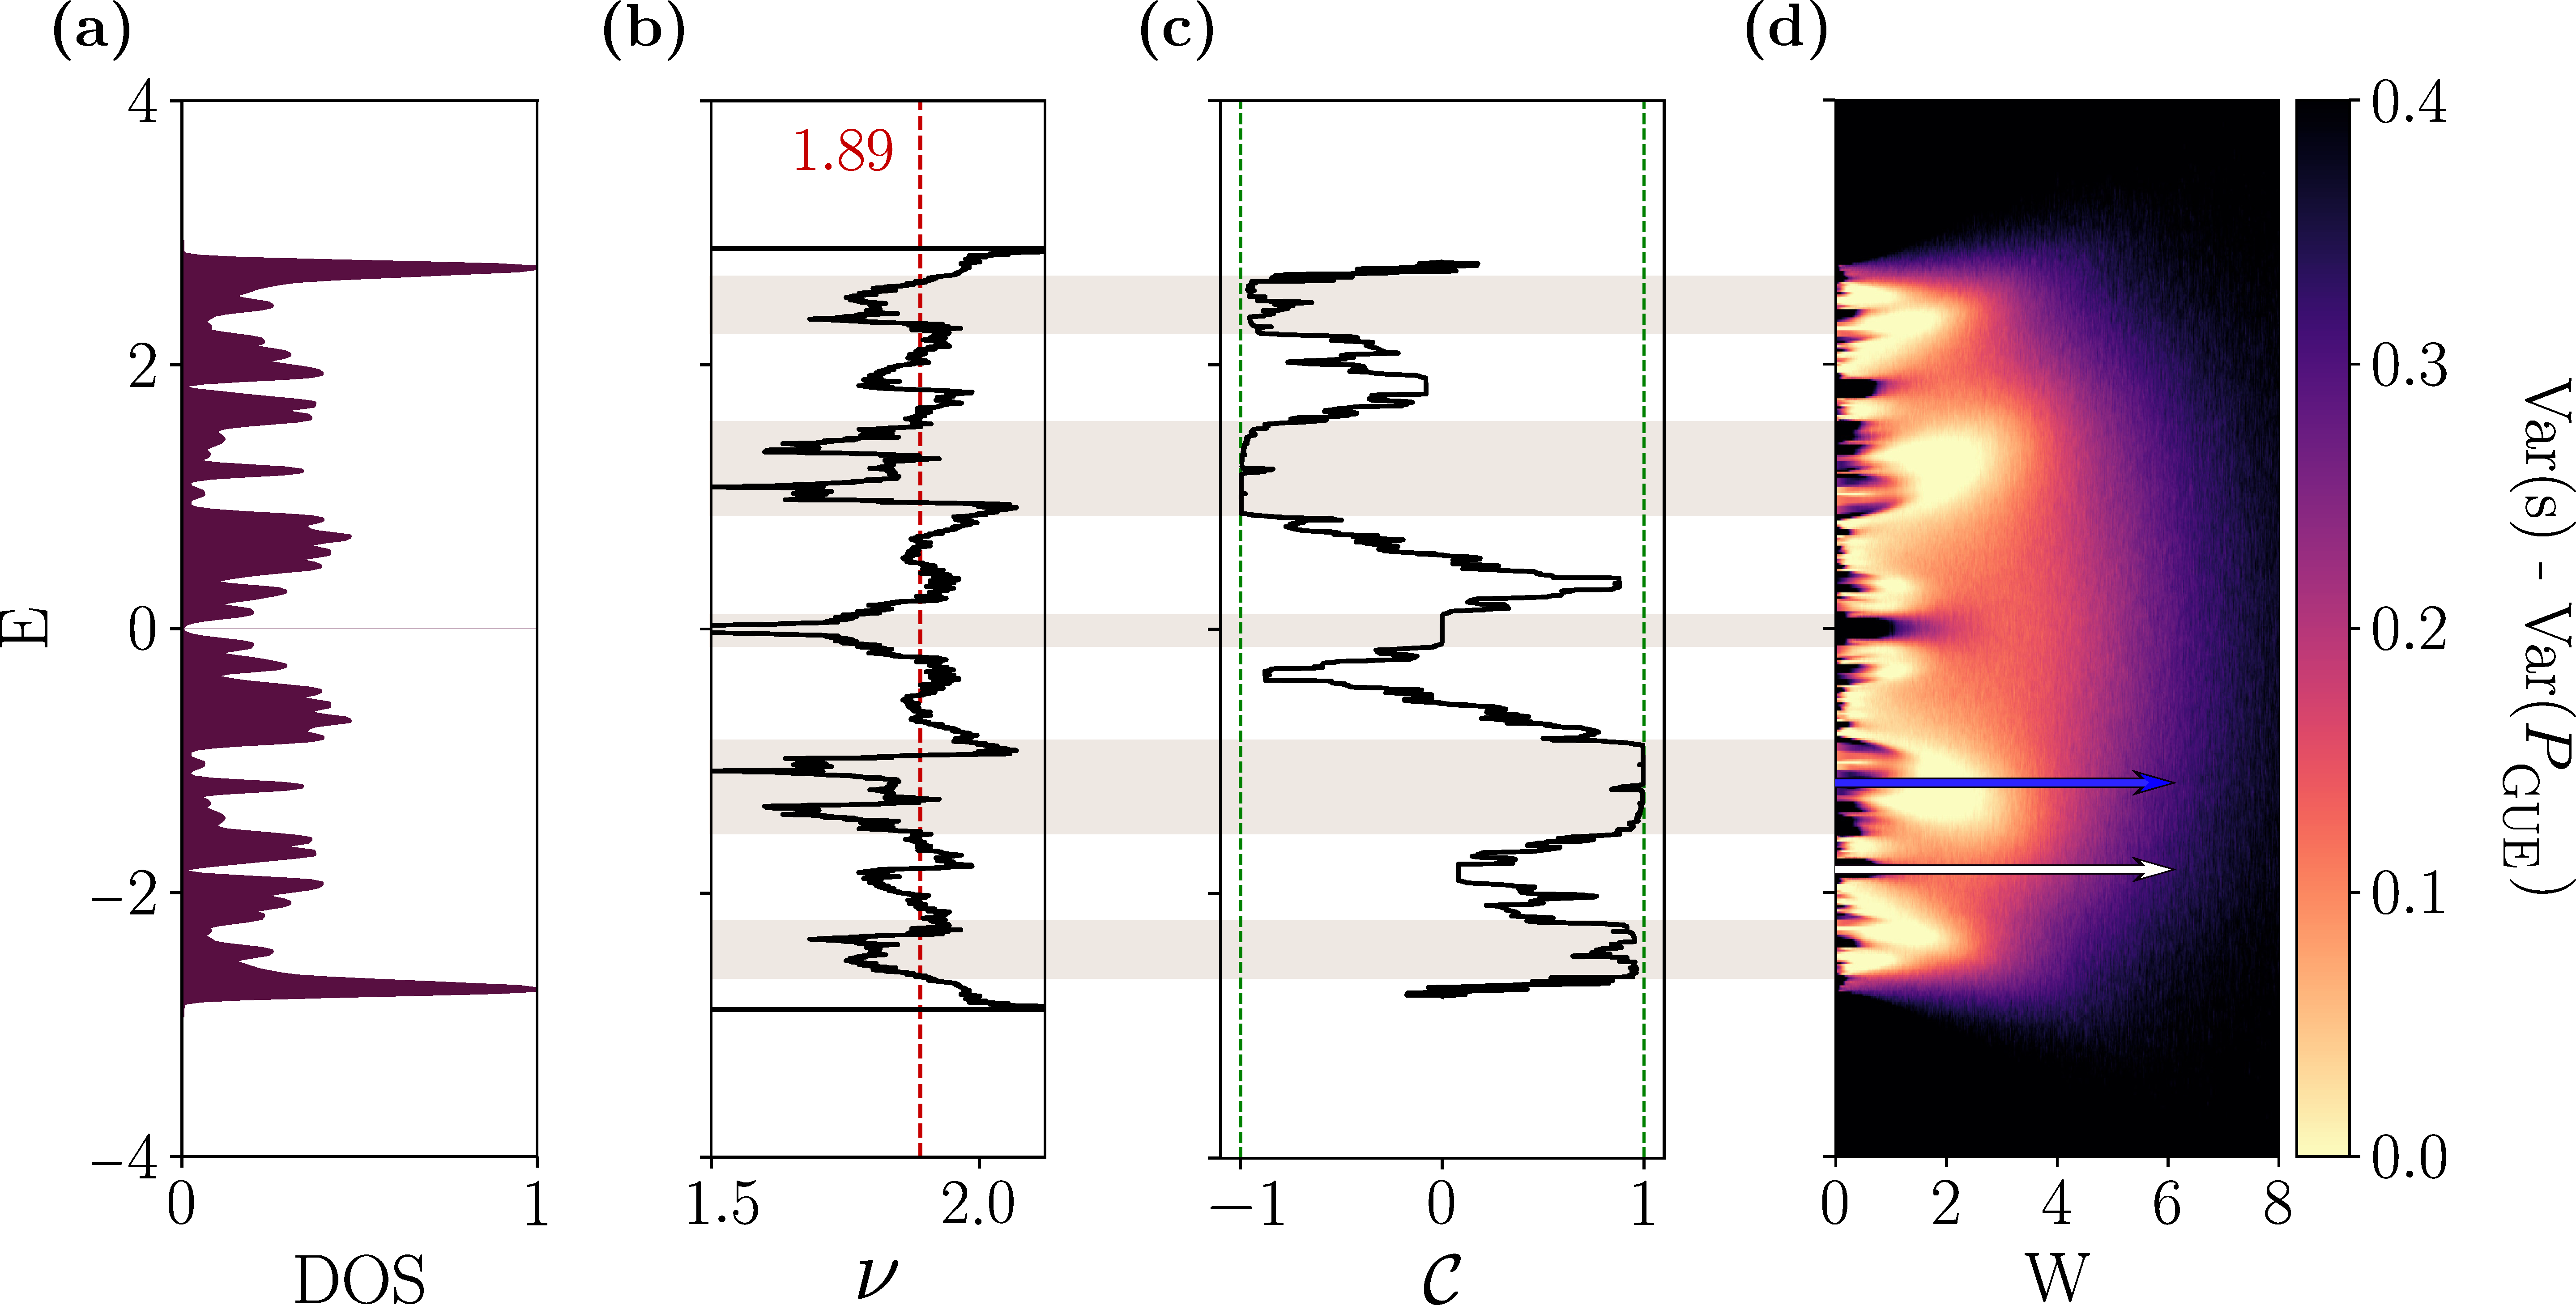
\includegraphics[width=0.95\textwidth]{frac_SC.pdf} 
\caption[Topological properties of the Sierpiński carpet at fixed flux $\alpha = 1/4$]{Topological properties of Sierpiński carpet at fixed flux $\alpha = 1/4$: \textbf{(a)} density of states, \textbf{(b)} scaling exponent $\nu$ of the DOS with system size, \textbf{(c)} Chern number as a function of $E$ and \textbf{(d)} variance of level spacings in the energy-disorder strength plane. Grey rectangles are guide to the eye. We identify the full energy gaps to be trivial. Regions with quantized values of the Chern number close to 1 are separated by a delocalized state from the Anderson insulator limit (see blue arrow in \textbf{(d)}), which is a feature of quantum Hall states. This is in contrast to a direct transition to a fully localized phase for states carrying zero Chern number as a function of $W$ (white arrow in \textbf{(d)}). Regions with $\mathcal{C} \neq 0$ are characterized by a DOS scaling exponent $\nu$ smaller than $d_{H}$ in \textbf{(b)}.}
\label{fig:frac_SC}
\end{figure}

\begin{figure}[H]
\centering
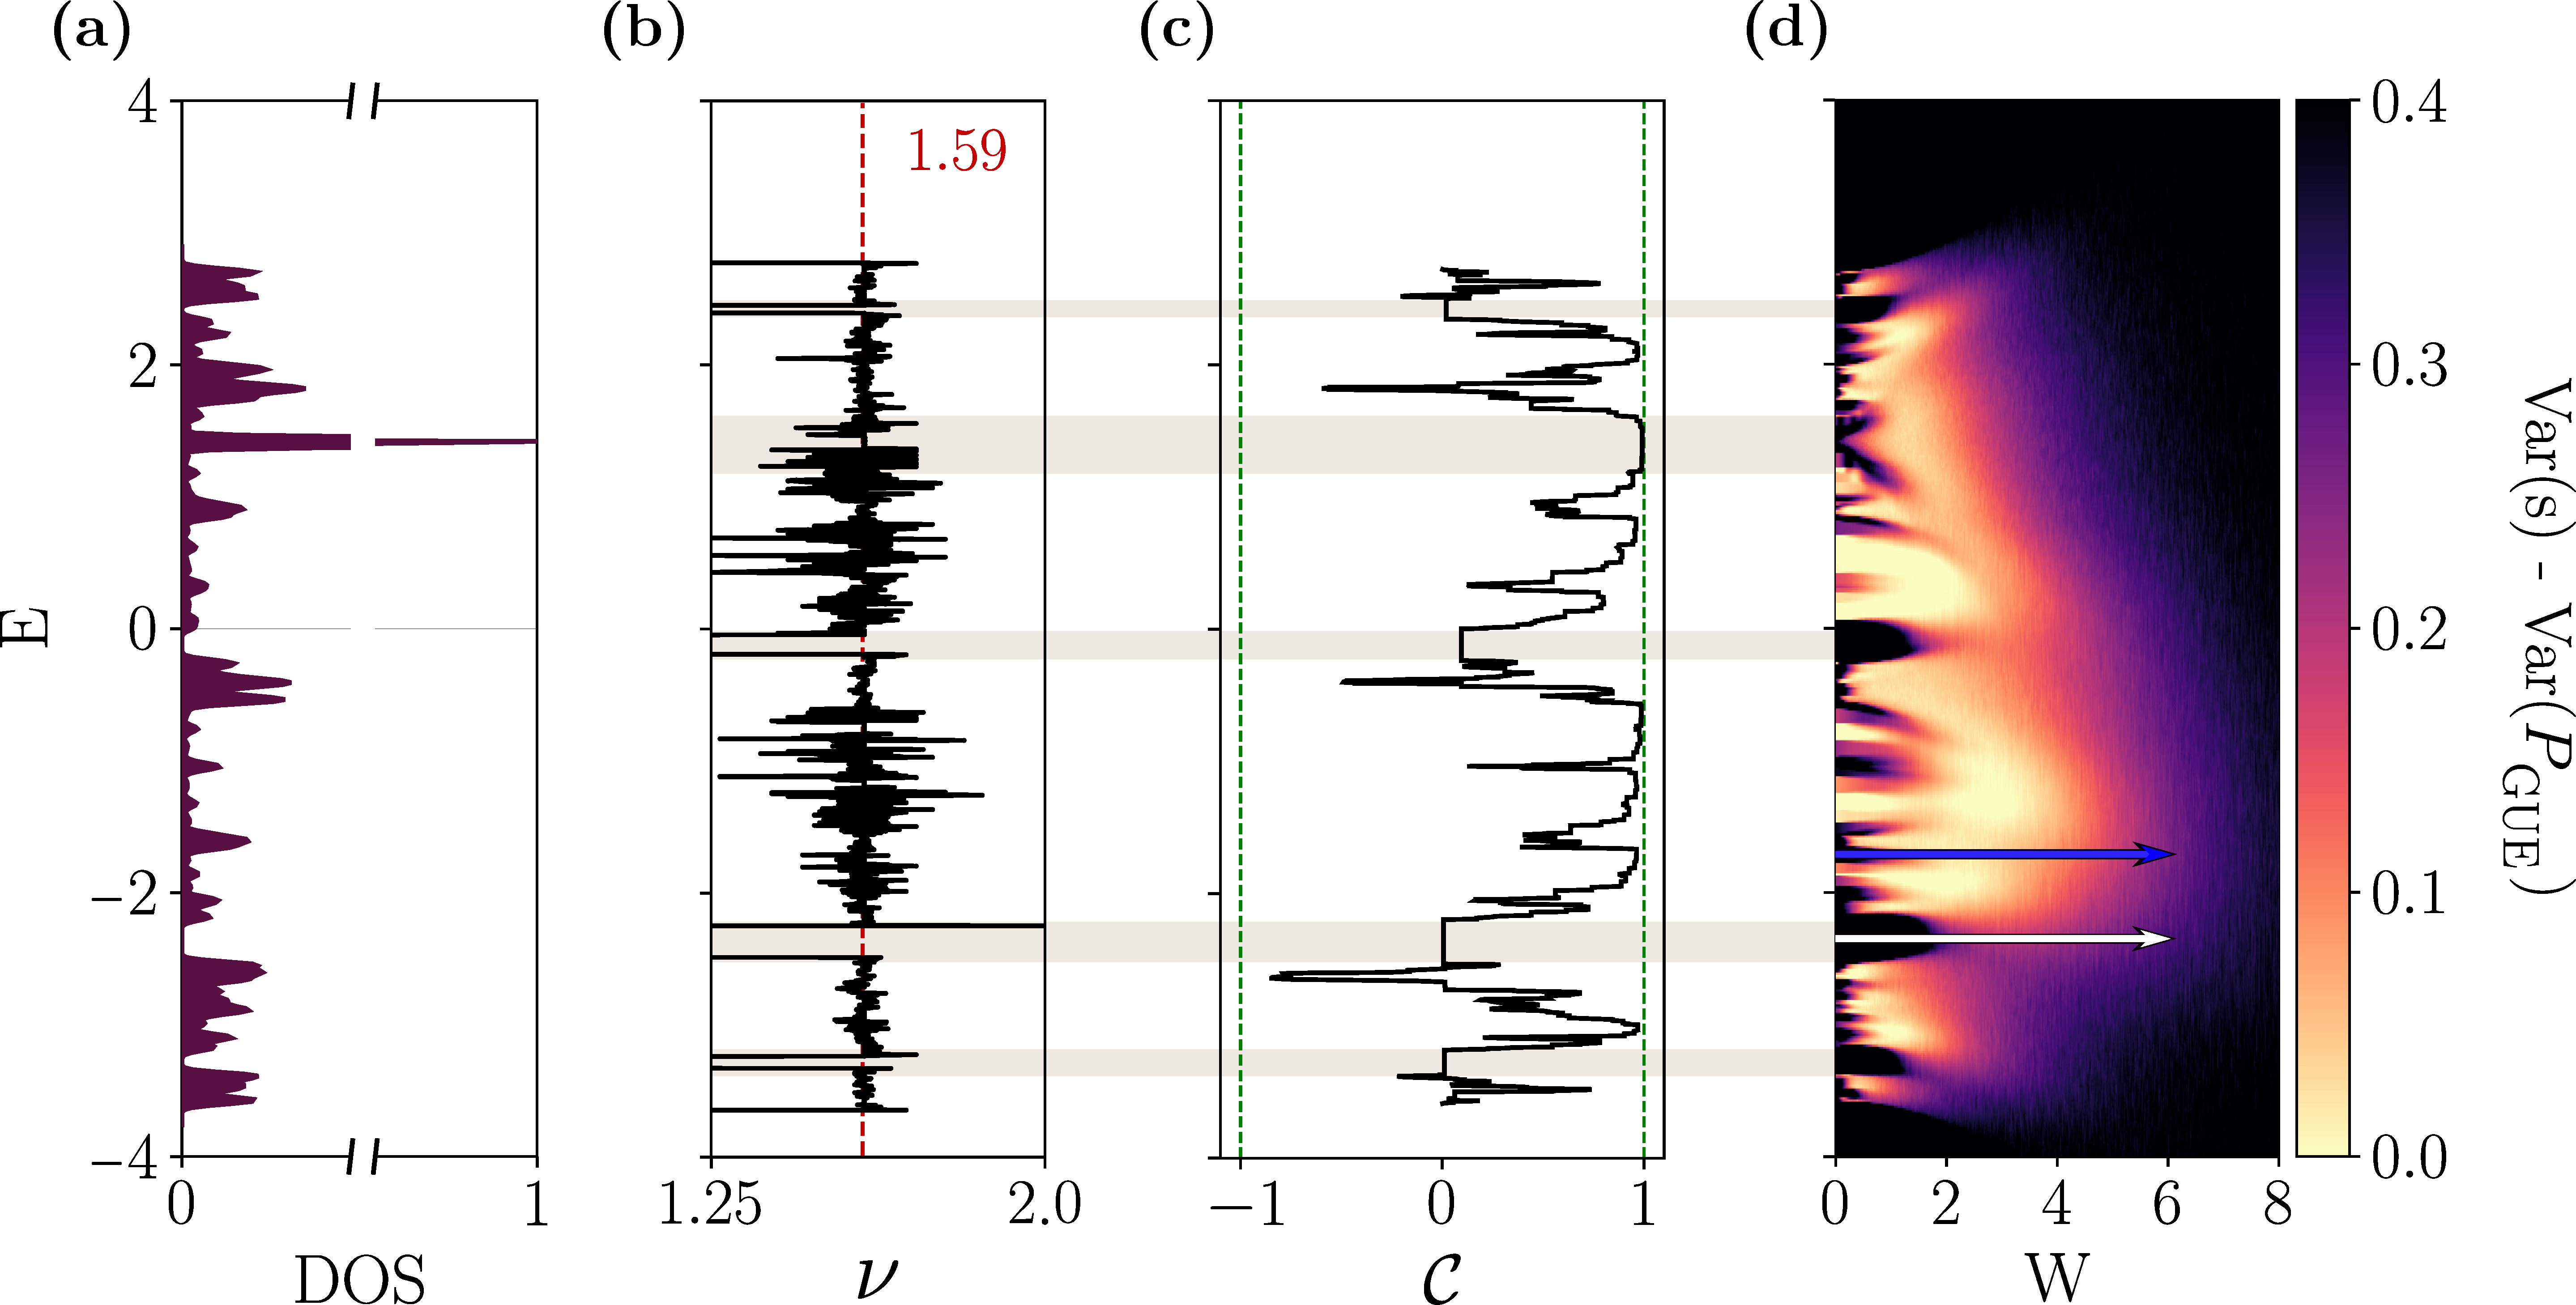
\includegraphics[width=0.95\textwidth]{frac_SG.pdf} 
\caption[Topological properties of the Sierpiński gasket at fixed flux $\alpha = 1/4$]{Topological properties of the Sierpiński gasket at fixed flux $\alpha = 1/4$: \textbf{(a)} density of states, \textbf{(b)} scaling exponent $\nu$ of the DOS with system size, \textbf{(c)} Chern number as a function of $E$ and \textbf{(d)} variance of level spacings in the energy-disorder strength plane. Similar to the SC, spectral gaps are also topologically trivial. Quantization of the Chern number is less pronounced, but the levitation and pair annihilation mechanism is still observed (see \textbf{(d)}).}
\label{fig:frac_SG}
\end{figure}

It is not obvious whether for fractals $\mathcal{C}$ tends to quantized values for almost all energies in the thermodynamic limit, that is the deviation from quantized $\mathcal{C}$ is solely due to finite-size effects. Because of the exponential increase in size for every iteration, performing systematic finite-size studies remains challenging. In the follow-up works on the SC~\cite{EdgesFremling2020, KatnelsonFractal2020}, the authors noted that the Hall conductivity $\sigma_{xy}$ is not quantized and not necessarily proportional to $\mathcal{C}$, but vary with the depth of the fractal. On the other hand, the edge states corresponding to non-zero $\sigma_{xy}$ are always present for a finite field strength and stable as one approaches the thermodynamic limit.

To discuss the connection between the DOS and the Chern number, we calculate the number of states at fixed flux $\alpha$ averaged over an energy interval $[\epsilon - \delta,\, \epsilon + \delta]$ (with $\delta = 0.1$ for the SC and $\delta = 0.05$ for the SG) for different system sizes, and compute the average scaling exponent $\nu$ of the number of states in that energy range with system size. On average, $\nu$ equals the Hausdorff dimension $d_{H}$. In Fig.~\ref{fig:frac_SC}~(b), we see that for the SC regions with a (nearly) quantized Chern number consistently show scaling with $\nu < d_{H}$. This indicates that the normalized DOS would scale to zero in the thermodynamic limit in regions with quantized Chern number. For the SG, the situation is less clear except in regions of trivial Chern number where no states are found (see Fig.~\ref{fig:frac_SG}~(b)). 

An important comment has to be made on the discrepancies between the Bott index and the Chern number calculations, especially in case of the SG. Firstly, we would like to point out that larger lattices were investigated with local markers, hence the self-similar structure of energy spectrum is more complex and new subregions associated with a non-trivial topological index appear. In finite systems, it is not guaranteed that the Bott index is equivalent to the Chern number; yet, an agreement may be expected for larger, not necessarily numerically tractable, system sizes.

%%%%%%%%%%%%%%%%%%%%%%%%%%%%%%%%%%%%%%%%%%%%%%%%%%%%%%%%%%%%%%%%%%%%%%%%%%%%%%%%%%%%%%%%%%%%%%%%%%%%%%%%%%%%%%%%%%%%%%%%
\subsection{Effect of disorder}
Topological matter is often defined in terms of its immunity to disorder. As suggested by Anderson~\cite{anderson}, a constructive quantum interference between wavefunctions of particles may result in localization by a random potential. However, if carriers move along one edge of the sample, the physical separation between pairs of opposite edge channels precludes backscattering. This property underlies the robustness of topological systems. In QH setups, disorder splits the degeneracy of the bulk Landau levels, but the edge modes remain unaffected - because of their chirality, they cannot scatter in a single edge channel and scattering between edges is exponentially suppressed. Sufficiently strong disorder destroys this physical picture and the system enters into a global insulating phase~\cite{PhysRevLett.78.318}.

For this reason, we would like to investigate the effect of disorder by adding extra term $\sum_i V_i c_i^{\dagger} c_i$ to the Hamiltonian defined in Eq.~\eqref{eq:frac_ham}, where $V_i$ is drawn from a uniform distribution $\left[ -W/2, W/2 \right]$ and $W$ corresponds to the disorder strength. If the system is initially characterized by a non-vanishing Hall conductivity, introducing disorder does not lead to an instant transition to a trivial Anderson phase, where all states, including the protected boundary modes, are fully localized at lattice sites. Instead, a disorder-induced topological phase transition is accompanied by a so-called levitation and pair annihilation mechanism~\cite{PhysRevLett.52.2304, onoda}. As the disorder increases, the states characterized by non-zero Chern number move towards each other, they meet at intermediate disorder values and annihilate, ultimately leading to Anderson localization at large disorder strength exceeding the band width. Notably, the edge states are rather protected by the mobility gap -- an interval in the spectrum of a Hamiltonian between mobility edges that are separating regions of localized and extended states, than by the band gap as in typical topological band insulators. Such protection is observed, for instance, in the topological Anderson insulators, where the disorder gives rise to the non-trivial topology~\cite{PhysRevLett.102.136806, PhysRevLett.103.196805}.

Potential disorder-induced transition can be captured by level spacing defined as the difference between neighbouring energy levels. For a given energy $\epsilon$ and disorder realization $\{V_i\}$, we find two closest eigenvalues satisfying $ E_{\lambda, \{V_i\}} < \epsilon < E_{\lambda + 1, \{V_i\}}$, then calculate level spacings 
\begin{equation}
s_{\epsilon, m, \{V_i\}} = E_{\lambda + m + 1, \{V_i\}} - E_{\lambda + m, \{V_i\}}, 
\label{eq:levelspacing}
\end{equation}
where $m \in \lbrace -k, k \rbrace$, and normalize them. We set $k = 2$ as proposed in Refs.~\cite{2010:ProdanDisordCI, 2011:Prodan} and point out that incorporating differences between further neighbouring levels does not affect the results. Hence, we can study the distribution of the level spacings and the variance $\mathrm{Var} (s_{\epsilon}) = \langle s_{\epsilon}^2 \rangle - \langle s_{\epsilon} \rangle^2$ to determine whether states are localized or extended. The average is taken over $m$ and $10^3$ disorder realizations for fixed $\epsilon$. According to random matrix theory, Hamiltonians with broken time-reversal symmetry are modelled by the Gaussian unitary ensemble (GUE). If the states are delocalized, then the level spacings should follow the Wigner-Dyson distribution $P_{\mathrm{GUE}} (s) = \frac{32 s^2}{\pi^2} e^{-\frac{4}{\pi} s^2}$ with variance $\mathrm{Var}(P_{\mathrm{GUE}}) = 0.178$. Localized states, on the other hand, are expected to obey the Poisson distribution $P (s) = \exp (-s)$ with a large variance $ \sim \mathcal{O}(1)$. Consequently, we study the numerically obtained distributions of the level spacings for several disorder amplitudes $W$ and compute the variance in order to demarcate between localized and delocalized states. Exemplary distributions are illustrated in Figs.~\ref{fig:SC_levels} and \ref{fig:SG_levels}.

\begin{figure}[H]
\centering
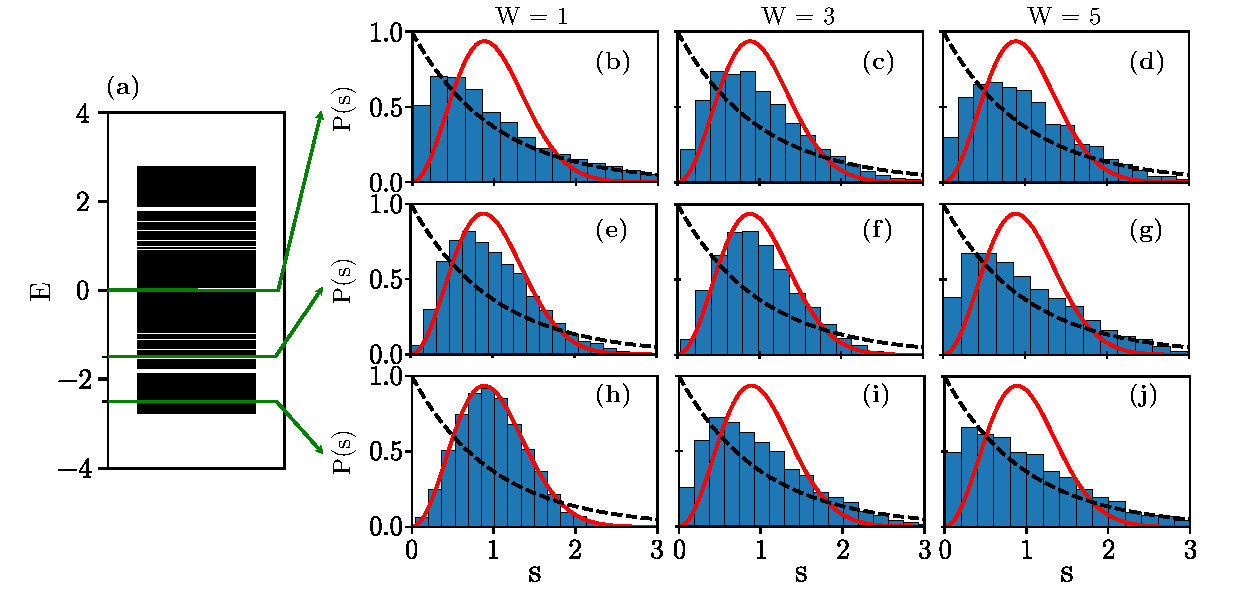
\includegraphics[width = \textwidth]{frac_SC_levels.pdf}
\caption[Distribution of level spacings for Sierpiński carpet at different disorder strengths]{\textbf{(a)} Energy spectrum for the clean carpet at flux $\alpha = 1/4$, \textbf{(b) - (j)} distributions of the level spacings compared to GUE (red solid line) and Poisson (black dashed line). Set of histograms correspond to the energy around: $\epsilon = 0$ \textbf{(b, c, d)}, $\epsilon = -1.5$  \textbf{(e, f, g)}, $\epsilon = -2.5$ \textbf{(h, i, j)}.}
\label{fig:SC_levels}
\end{figure}

\begin{figure}[H]
\centering
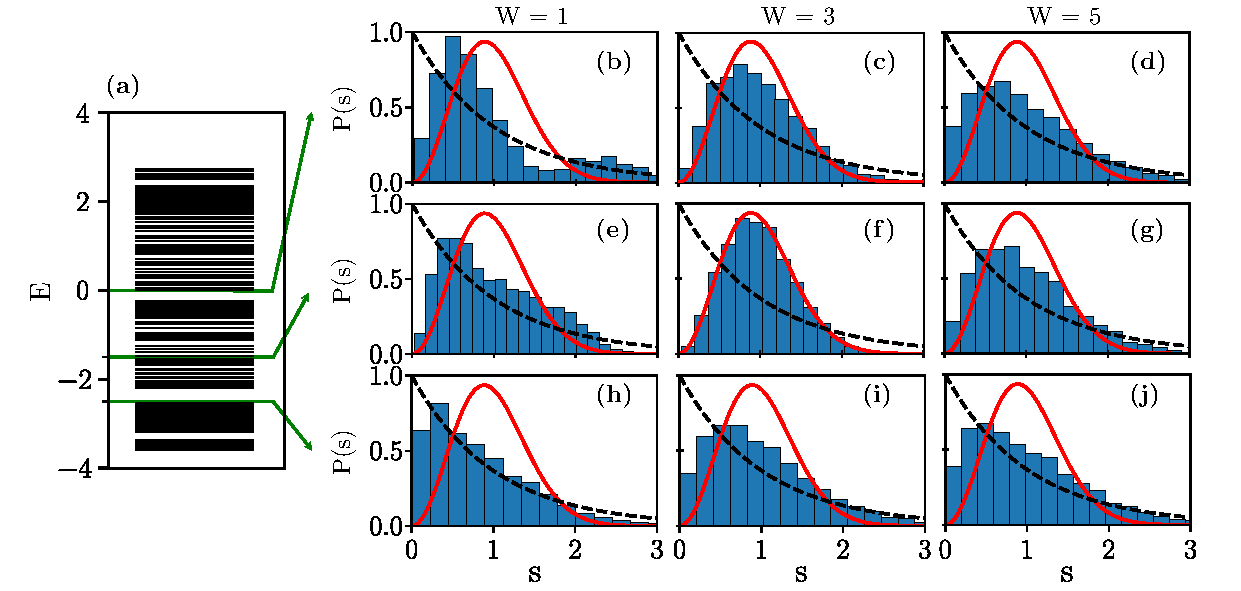
\includegraphics[width = \textwidth]{frac_SG_levels.pdf}
\caption[Distribution of level spacings for Sierpiński gasket at different disorder strengths]{\textbf{(a)} Energy spectrum for the clean gasket at flux $\alpha = 1/4$, \textbf{(b) - (j)} distributions of the level spacings compared to GUE and Poisson statistics denoted by red solid and black dashed lines, respectively. Set of histograms correspond to the energy around: $\epsilon = 0$ \textbf{(b, c, d)}, $\epsilon = -1.5$  \textbf{(e, f, g)}, $\epsilon = -2.5$ \textbf{(h, i, j)}.}
\label{fig:SG_levels}
\end{figure}

Since disorder calculations require exact diagonalization of the Hamiltonian repeatedly, we consider here smaller systems (iteration $n = 3$ in case of SC and $n = 5$ for SG). This is justified by the fact that fractals exhibit the same statistical properties at different scales. In Figs.~\ref{fig:frac_SC} (d) and \ref{fig:frac_SG} (d), we present the difference between $\mathrm{Var (s)}$ and $\mathrm{Var}(P_{\mathrm{GUE}})$ at fixed flux $\alpha = 1/4$. Regions in energy for which the Chern number is quantized are characterized by a large $\mathrm{Var} (s)$ at small values of $W$. There are two possible transition scenarios, which can be observed by following a line of increasing $W$ at constant energy, represented by white and blue arrows. The former case corresponds to a direct transition to a fully localized system, without $\mathrm{Var} (s)$ ever becoming close to $\mathrm{Var}(P_{\mathrm{GUE}}) = 0.178$. In the latter case, a localized region at small $W$ is separated from the Anderson insulating limit by a delocalized region with $\mathrm{Var}(P_{\mathrm{GUE}}) = 0.178$. 

\begin{figure}[H]
\centering
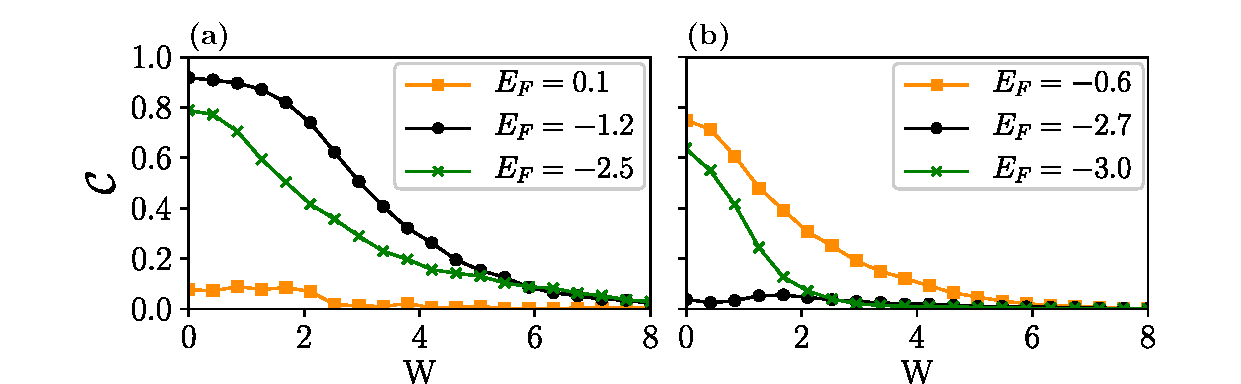
\includegraphics[width = \textwidth]{frac_chern_disord.pdf}
\caption[Chern number as a function of disorder]{Chern number as a function of disorder strength for \textbf{(a)} the carpet and \textbf{(b)} the gasket at fixed flux $\alpha = 1/4$ and three different Fermi levels corresponding to the parts of energy spectra with different degree of quantization of $\mathcal{C}$. For states characterized by the Chern number close to quantized non-zero value in the clean limit, $\mathcal{C}$ is larger than zero in a presence of moderate disorder and slowly reaches zero in the strong disorder regime.}
\label{fig:chern_disorder}
\end{figure}

\begin{figure}[H]
\centering
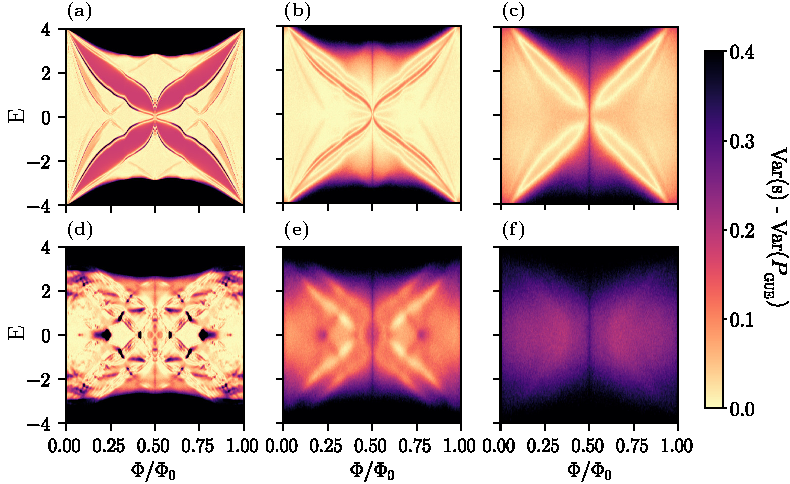
\includegraphics[width = 0.95\textwidth]{frac_square_sc.pdf}
\caption[Variance of the level spacings for a square lattice and the Sierpiński carpet at different disorder strengths]{Variance of the level spacings for \textbf{(a, b, c)} a square lattice and \textbf{(d, e, f)} the Sierpiński carpet in the energy - flux plane at three disorder strengths: \textbf{(a, d)} $W = 1$,  \textbf{(b, e)} $W = 3$, and \textbf{(c, f)} $W = 5$. At small disorder, $W = 1$, a model defined on a square lattice hosts delocalized states, which are separated by low DOS regions with a larger value of $\mathrm{Var} (s)$. For the SC, however, this separation is less clear. While increasing $W$, both systems undergo a transition through a point where all states become delocalized. A stronger disorder is needed to enter an Anderson insulating limit in case of a square lattice.}
\label{fig:var_SC_square}
\end{figure}

In Fig.~\ref{fig:chern_disorder}, we show the Chern number averaged over $300$ disorder realizations with respect to disorder strength $W$ for three different Fermi levels. For states characterized by $\mathcal{C}$ close to one in the absence of disorder, the Chern number remains non-zero in a moderate disorder regime. At the same time, states with initially almost zero $\mathcal{C}$ stay near this value (up to small fluctuations). We conclude that in the energy regions where the Chern number is close to one, the topological features survive small disorder. As expected, in the Anderson insulating phase, $\mathcal{C}$ vanishes for all states.

As a cross-check of our calculations, we compare the variances of the level spacings computed over the whole flux range at three different disorder strengths $W = 1, \, 3, \, 5$ for regular and fractal lattices (results are illustrated in Figs.~\ref{fig:var_SC_square} and \ref{fig:var_SG_triangle}). In case of a square and the SC in a presence of moderate disorder, a large variance along a line $\alpha = 1/2$ is observed as systems become time-reversal invariant. In general, topological features in fractal lattices are less robust to disorder than in regular lattices.

\begin{figure}[H]
\centering
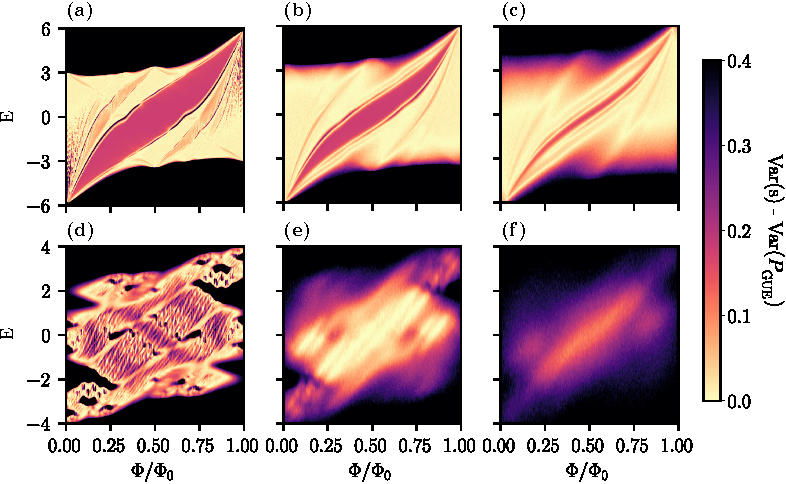
\includegraphics[width = 0.95\textwidth]{frac_triangle_sg.pdf}
\caption[Variance of the level spacing for a triangular lattice and the Sierpiński gasket at different disorder strengths]{Variance of the level spacings for \textbf{(a, b, c)} a triangular lattice and \textbf{(d, e, f)} the Sierpiński gasket in the energy - flux plane at three disorder strengths: \textbf{(a, d)} $W = 1$,  \textbf{(b, e)} $W = 3$, and \textbf{(c, f)} $W = 5$. In case of a triangular lattice, delocalized states are separated by the mobility gap, which decreases with respect to $W$. In contrast, the SG exhibits numerous small localized regions at $W =1$, which ultimately become a one delocalized region at $W =3$.}
\label{fig:var_SG_triangle}
\end{figure}